 \documentclass [12pt]{article}
\usepackage{geometry}
 \geometry{
 a4paper,
 left=25mm,
 right=25mm,
 top=30mm,
 bottom=30mm,
 headsep=10mm,
 footskip=15mm}
\linespread{1.175}\selectfont
\usepackage{blindtext}
\usepackage[utf8]{inputenc}
\usepackage[english]{babel}
\usepackage{lipsum}
\def\labelitemi{--}
\def\labelitemii{*}
\pagenumbering{arabic}
\usepackage[hidelinks]{hyperref}
\usepackage{fancyhdr}
\usepackage[shortlabels]{enumitem}
\usepackage{wrapfig}
\pagestyle{fancy}
\fancyhf{}
\lhead{\small{Bealthy project by Meneghin Giulia \& Mauri Giuseppe}}
\rhead{\small{\rightmark}}
\rfoot{\small{Page \thepage}}
\lfoot{\small{Copyright © 2020, Meneghin Giulia \& Mauri Giuseppe  – All rights reserved}}

\setlength{\headheight}{17pt}
\usepackage{graphicx}
\newcommand{\sectionbreak}{\clearpage}
\usepackage{titlesec}
\usepackage{hyperref}
\usepackage{subcaption}
\usepackage{tabu}
\begin{document}

\begin{figure}[ht!]
\centering

\includegraphics[height=5.8cm,width=5.8cm]{logopoli.png}
\end{figure}
\begin{large}
\centerline{\textbf{Politecnico di Milano} }
\centerline{AA 2020-2021}
\vspace{0.5cm}
\centerline{Design and Implementation of Mobile Applications}
\centerline{\textbf{Dima}}
\end{large}
\begin{figure}[ht!]
\centering

\includegraphics[width=\linewidth]{Immaginecopertina.png}
\end{figure} 

\clearpage

\begin{table}[h!]
\begin{tabu} to \textwidth { X[0.3,r,p] X[0.7,l,p] }
\hline

\textbf{Deliverable:} & DD\\
\textbf{Title:} & Design Document \\
\textbf{Authors:} & Meneghin Giulia \& Mauri Giuseppe \\
\textbf{Version:} & 1.0 \\ 
\textbf{Date:} & 05-January-2021 \\
\textbf{Download page:} & \url{<https://github.com/Ciuse/MauriMeneghin>} \\
\textbf{Copyright:} & Copyright © 2020, Meneghin Giulia \& Mauri Giuseppe – All rights reserved \\
\hline
\end{tabu}
\end{table}

\clearpage

\tableofcontents

\section{Introduction}
\subsection{Scope}
Bealthy is an application that allows the user to enter the dishes they consume and monitor the symptoms they experience on a daily basis. 
The entry of dishes can be done by: searching a predefined list of foods known to our application, scanning a barcode with the camera, or manually entering the information of the dish.
The purpose of the application is to collect the data entered by the user, process it and reorganize it in the form of a graph to show the user the correlation between the symptoms experienced and the individual ingredients consumed.
The application implements three types of graphs:
The first consists of showing which symptoms/ingredients have a higher percentage of the total in a specific period of days.
The second type shows which ingredients affect a particular symptom in the selected time period.
The third shows of an ingredient what is the likelihood of causing one or more symptoms.
In addition, the system allows the user to enter his or her medical treatments that he or she is following and shows past treatments.
The system compares the previous month's symptom data with that of the days under treatment to show the effectiveness of the treatment taken.
\subsection{Goals}
\begin{enumerate}
\item[(G1)]Allow the user of the application to create a personal account and modify his information.
\item[(G2)]Allow the user to change the current day with an interactive calendar.
\item[(G3)]Allow the user to add a dish to a specific mealtime of the selected day(Breakfast, Lunch, Snack, Dinner), setting the eaten quantity.
\item[(G4)]Allow the user to search a dish.
\item[(G5)]Allow the user to scanning a bar code with the camera application.
\item[(G6)]Allow the user to create a new dish with a specific image and a lists of ingredients. 
\item[(G7)]Allow the user to add a symptom in a specific day, setting the intensity, frequency, mealtime occurrences.
\item[(G8)]Allow the user to delete the inserted dishes.
\item[(G9)]Allow the user to delete the inserted symptoms.
\item[(G10)]Allow the user to visualize the percentage of symptoms occurrences and ingredients eaten in a fixed days range (weekly or monthly) or in a days range selected with the calendar.
\item[(G11)]Allow the user to visualize the correlation between the symptoms occurrences and the eaten ingredients.
\item[(G12)]Allow the user to visualize a page tha shows of an ingredient what is the likelihood of causing one or more symptoms.
\item[(G13)]Allow the user to visualize the in progress treatments and the completed ones.
\item[(G14)]Allow the user to add a new treatment specifying the diet and medical cure.
\item[(G15)]Allow the user to remove a treatment.
\item[(G16)]Allow the user to change the profile image.


\end{enumerate}
\subsection{Functional Requirement}
\begin{description}
\item[(G1)]Allow the user of the application to create a personal account with an email and password, or with an external services (Google, Github, Twitter).
\begin{itemize}
\item The user should be able to register through the mobile application and in order to do that he has to provide a password, and a valid e-mail.\\
\end{itemize}
\end{description}

\begin{description}
\item[(G2)]Allow the user to change the current day
\begin{itemize}
\item  by clicking another day on the interactive calendar.
\item by using the appropriate tab to change the dates.
\end{itemize}
\end{description}

\begin{description}
\item[(G3)]Allow the user to add a new dish in a specific mealtime.
\begin{itemize}
\item The user has to click on the "+" button of the mealtime he/she has chosen to add a new dish.
\item  Then he/she can choose the way with which adding the dish. There are 5 ways to add it:\\
\item[(G4)] The first 3 ways consist of searching for the dish:
\begin{itemize}[•]
\item Using the \textbf{"Search list"} button:\\
A list of all the dishes in the online database will appear. After selecting the desired dish and entering the quantity eaten, it will be automatically inserted on the Homepage in the box corresponding to the previously selected mealtime.
\item Using the \textbf{"Favourites list"} button:\\
A user list of all favourites dishes will appear. After selecting the desired dish and entering the quantity eaten, it will be automatically inserted on the Homepage in the box corresponding to the previously selected mealtime. 
\item Using the \textbf{"Your created dishes list"} button:\\
A user list of all created dishes will appear. After selecting the desired dish and entering the quantity eaten, it will be automatically inserted on the Homepage in the box corresponding to the previously selected mealtime.
\end{itemize}

\item[(G5)] Using the \textbf{"Scanning a barcode"} button:\\
The user can scan the product eaten and if there is a valid match in the external database "Open food facts" the page containing all the information about it will be shown.  The user can edit the image, the name and the list of ingredients provided. Once the quantity eaten has been entered, it will be automatically inserted on the Homepage in the box corresponding to the previously selected mealtime.
\item[(G6)] Using the \textbf{"Creating new dish"} button:\\
A form for manually entering the information of the dish eaten will appear: 
The user can enter a picture (using the mobile camera or uploading it from own image gallery), a name, the quantity eaten and the ingredients with their corresponding quantity.The user must then click on the "create" button to create it and add it on the Homepage in the box corresponding to the previously selected mealtime. 
\end{itemize}
\end{description}

\begin{description}
\item[(G7)]Allow the user to add a symptom in the selected day
\begin{itemize}
\item The user has to click on the "+" button in the symptom box of the HomePage.
\item A page with all symptoms provided by the system will open and after clicking on the symptom that the user wants, another page will open.
\item the user has to set the various parameters required: the intensity of the perceived pain, the frequency with which the symptom occurred and the time(s) of day it occurred. 
\item Once you have entered all the parameters, the "save" button will become clickable. The user can click on this button to automatically add the symptom to the Homepage.
\end{itemize}
\end{description}

\begin{description}
\item[(G8)]Allow the user to delete a dish
\begin{itemize}
\item The user has to click on the dish button to remove its occurrence from a specific time of the selected day. 
\item On the page with the specific information of that dish, there is a "delete" button on the top right corner of top app bar. The user has to click on it.
\end{itemize}
\end{description}

\begin{description}
\item[(G9)]Allow the user to remove a symptom occurrence from a specific day
\begin{itemize}
\item The user must click on the symptom button in the Homepage to remove its occurrence. 
\item On the page with the specific information of that symptom, there is a button to reset all parameters, so the user can delete it.
\end{itemize}
\end{description}

\begin{description}
\item[(G10)]Allow the user to visualize the percentage of symptoms occurrences and ingredients eaten in a fixed days range (weekly or monthly) or in a days range selected with the calendar.
\begin{itemize}
\item The user has to select the statistics icon in the bottom app bar to view the graphs of symptoms and ingredients. 
\item By clicking the button in the top right corner of the app bar, he can change the period of days (week or month). 
\item In this page there are two Tabs that allow navigation between groups of content that are related and at the same level of hierarchy: symptoms and ingredients.
\begin{itemize}[•]
\item[(G11)] In the first tab "symptoms" there is a pie chart with the percentage of symptoms and under it, there are all the symptoms button. Clicking on one of them will open another bar graph showing the severity of that specific symptom during the selected period of days. Moving from one day to the next will show the list of ingredients that most caused that symptom.
\item[(G12)] In the second tab "ingredients" there is a pie chart with the percentage of ingredients and under it, there are all the ingredients button. Clicking on one of them will open another page that shows of an ingredient what is the likelihood of causing one or more symptoms.
\end{itemize}
\end{itemize}
\end{description}

\begin{description}
\item[(G13)]Allow the user to visualize the treatments in progress and the completed ones.
\begin{itemize}
\item The user has to select the treatments icon in the bottom app bar to open the page that shows the list of treatments in progress or that ones completed.  
\end{itemize}
\end{description}

\begin{description}
\item[(G14)]Allow the user to add a new treatment 
\begin{itemize}
\item The user has to select the treatments icon in the bottom app bar to open the page that shows the list of treatments in progress or that ones completed.  
\item In that page the user can click on the "+" button in order to create a new treatment.
\item Clicking on the button will open the page containing the form for entering a new treatment. The name, start date and end date of the treatment are compulsory, while the description, medical information and diet are optional.
\end{itemize}
\end{description}

\begin{description}
\item[(G15)]Allow the user to remove a treatment 
\begin{itemize}
\item The user has to select the treatments icon in the bottom app bar to open the page that shows the list of treatments in progress or that ones completed.  
\item In that page the user can click on the treatment he/she wants to delete.
\item In the page of treatment information, there is the "delete" button. The user has to click on it.
\end{itemize}
\end{description}

\clearpage

\begin{description}
\item[(G16)]Allow the user to change the profile image 
\begin{itemize}
\item The user has to select the personal info icon in the bottom app bar to open the page that shows the information and the settings of the user.  
\item In that page the user can click on "camera" button in order to change his/her image profile.
\item The user can take a photo or upload an image from his/her gallery.
\end{itemize}
\end{description}



\subsection{Acronyms}
\begin{itemize}
\item\textit{API:} Application Programming Interface.
\end{itemize}

\subsection{Revision history}
\begin{itemize}
\item Version 1.0
\end{itemize}


\section{Architectural Design}
\subsection{Overview}
Bealthy application has a two tier architecture.
\begin{figure}[ht!]
\centering
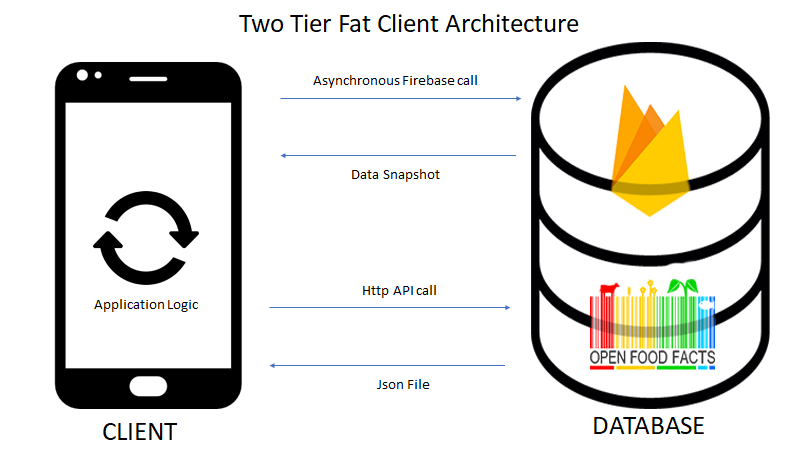
\includegraphics[height=8cm, width=\linewidth]{ArchitectureTwoTier.png}
\caption{Structure Overview} 
\end{figure}
\\
Bealthy uses a two tier architecture with a fat client. The client tier and the business logic tier are both located within the mobile application, while the database is remote. Most of the data are in the database managed by the provider "Firebase" on which there are all the static data of the predefined dishes, the dishes created by the user, the day by day information of which dishes he eats and which symptoms he shows, and the files of the images of the dishes and the photo of the user. The other part of the data is managed by the provider "OpenFoodFacts", an open source database containing thousands of food information associated with a barcode.

\subsection{High level components}
The architecture of the high-level components consists of two different types of elements:
the External Services and the Mobile Application.
\begin{itemize}
\item \textbf{The Mobile Application} allows users to interact directly with the system. This component provides a simple and clear view of the various functions that the system provides to the user. We decided to develop a fat client application that handles both the UI and UX part as well as the business logic. A fat client application  connects to a external remote database (firebase) in order to sync data or upload and download user information. 
Bealthy processes most of data by itself, it does not rely on any servers for processing. 
The processing of user data, in order to showing the correlation between the symptoms and the ingredients, is done offline.
\item There are two different kind of \textbf{External Services} that the application uses: The database ones and the authentication ones.
The external databases,Firebase and OpenFoodFact, are interrogated by our application when it needs their updated data while the external authentication services are: Google, Github and Twitter.
\end{itemize}

\subsection{Component view}
\subsubsection{High Level Widget structure}
\null
\vspace{\stretch{2}}
\begin{figure}[ht!]
\centering
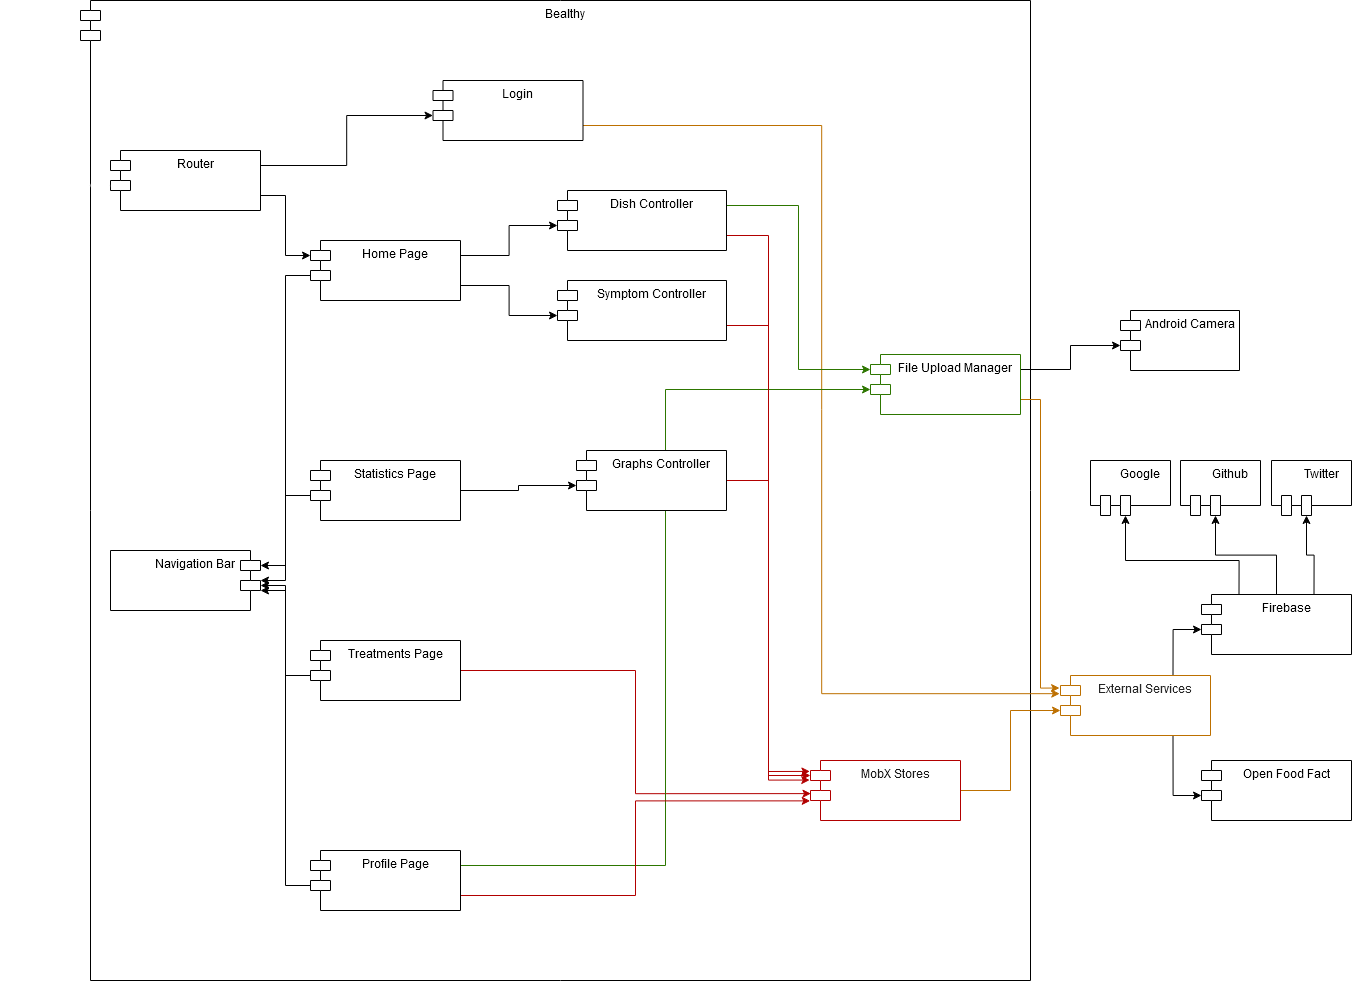
\includegraphics[height=14cm, width=\linewidth]{ComponentViewDiagram.png}
\caption{Widget Diagram}
\end{figure}  
\vspace{\stretch{5}}
\clearpage
The following diagram represents the main widgets that make up our application.
The first widget you have when you open the application is a router that redirects the view either to the login or to the home page based on whether you are already authenticated or not.
The login widget implements the methods and ui to allow the user to register and log in through the methods that Firebase provides.
The Main application instead consists of 4 main widgets, Home Page, Statistics Page, Treatment Page, and Profile Page, which are connected by a Bottom Navigation Bar.
The home page is linked to a widget that controls dishes (viewing and creation) and a widget that controls symptoms (viewing and creation).
The statistics page through a graph controller implements various widgets to show data in pie and bar graphs.
All widgets that deal with dynamic data are connected to a set of widgets enclosed in "Mobx Stores" which take care of holding the observable data and invoking functions to get it through Firebase and to update it locally once the response is received.
The profile and dishes pages are linked with a widget that handles all the part about getting a photo through the phone camera and uploading it to the Firestone Database.
\subsubsection{More detailed widget structure }
The diagram shows the main widgets that are used by the following Sequence diagrams.
This diagram shows the main widgets on our home page and the stores through which data is taken to be displayed as the day changes (explanation in sequence diagram number 1).
The other main widget that the diagram deals with is the page for adding a dish to a meal. The add screen has 5 other widgets.
In sequence diagram number 2 we treat the dish creation widget by highlighting the stores it uses to save the information on firebase of the new dish and to invoke the rebuild of the pages that will contain the newly created dish. In addition, the widget for creating a dish is connected to a component that manages the whole part related to take a picture with the phone camera.
\begin{figure}[ht!]
\centering
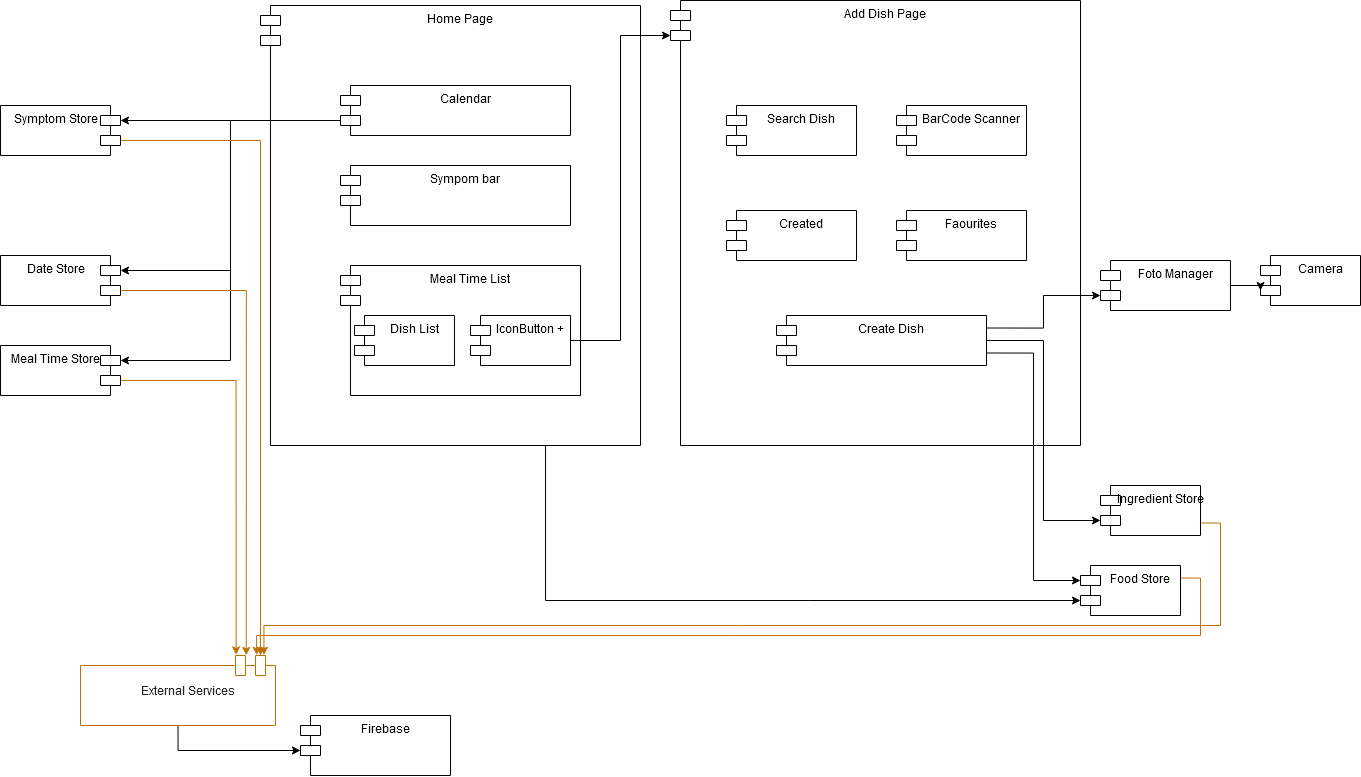
\includegraphics[height=14cm, width=\linewidth]{ComponentDettagliato.png}
\caption{more detailed widget diagram}
\end{figure}

\clearpage

\subsection{Runtime view}

\subsubsection{Sequence Diagram 1}
This sequence diagram illustrates what happens after the user changes the day through the calendar.
Clicking on a day in the calendar invokes a Date Store method that updates the observable variable containing the date with the selected date. This causes the UI to be notified of the change through Mobx. The home page reacts by rebuilding through the Observer Widget only the part of the calendar that has changed, while the Calendar reacts through a Mobx reaction by invoking two methods, one to update the list of dishes with those of the selected day, and the other to update the list of symptoms with the selected day.
The methods access the respective Store which invokes queries to firebase to get the data based on the selected day. Once the data is obtained the stores update the local observable lists triggering the Mobx notify which invokes in the UI a rebuild of the changed data through the Observers.

\begin{figure}[ht!]
\centering
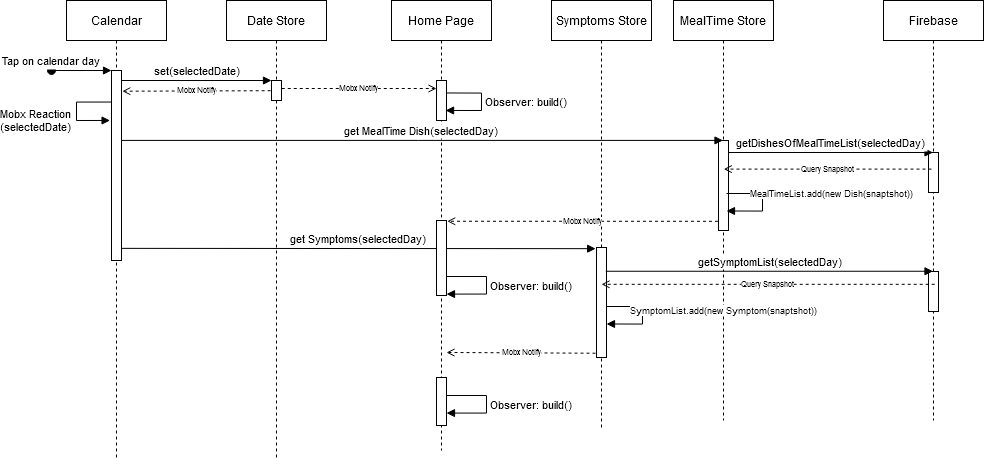
\includegraphics[height=19cm, width=\linewidth]{SequenceCalendarClick.png}
\caption{Sequence Diagram 1}
\end{figure}  
\clearpage
\subsubsection{Sequence Diagram 2}
This sequence diagram illustrates the steps for the user to create a new dish.
The action starts with the user pressing the "+" button on the homepage next to the "Breakfast" sign. The Navigator pushes the "Add Dish Page" in which the user presses on "Create Dish" and the Navigator pushes the "Create Dish" page.
In this last page the user will have to insert a photo of the dish, the name of the dish, and the ingredients of which it is composed.
Pressing on the camera icon invokes the Navigator which pushes the page where the user can take the photo, after agreeing to the permissions to use the camera. Once the photo is taken and the "Crop" is confirmed, the user clicks on Save Image and returns to the dish creation screen. 
Once all the data have been inserted and the "Create" button has been pressed, the form validator will check all the fields, and in the case of an error it will signal it to the user; while in the case of confirmation the Food Store will be invoked and once it has received the new dish created it will save it on Firebase, and update the list of local dishes, thus causing a rebuild through the MobX notify of the list of dishes observable on the homepage.
\begin{figure}[ht!]
\centering
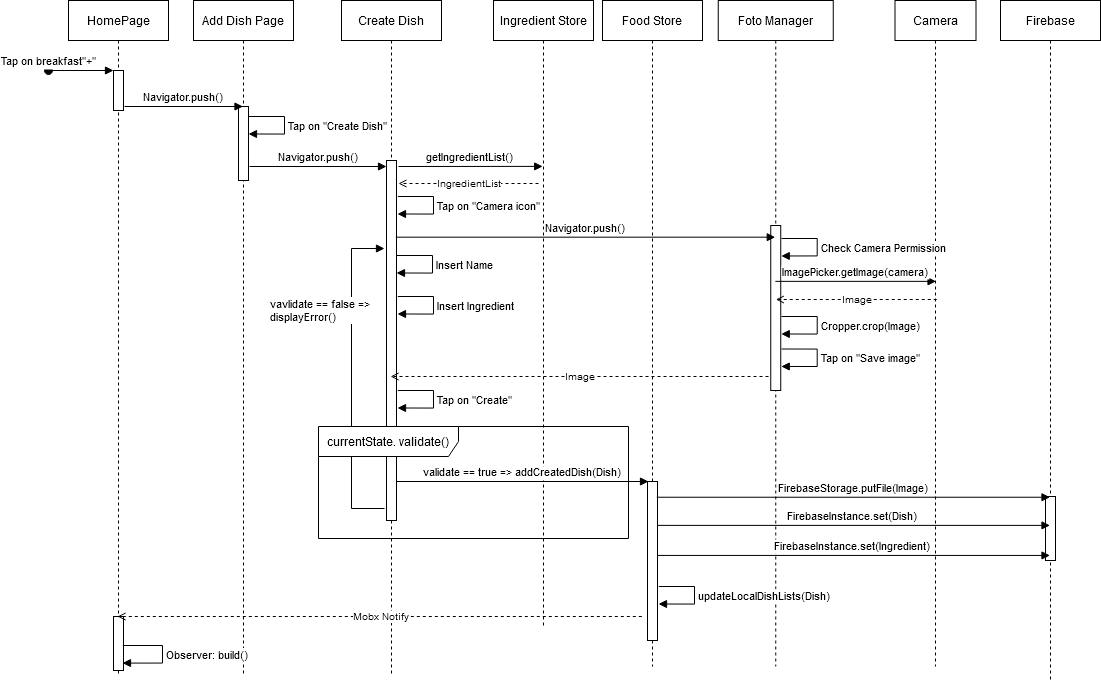
\includegraphics[height=19cm, width=\linewidth]{SequenceCreateDish.png}
\caption{Sequence Diagram 2}
\end{figure}  
\clearpage

\subsection{Styles and patterns}
\subsubsection{Overall Architecture}

\begin{figure}[ht!]
\centering
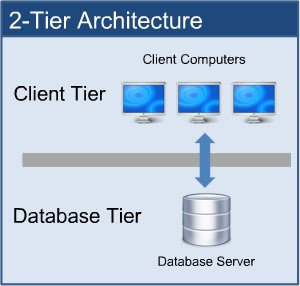
\includegraphics[height=7cm, width=7cm]{2tier.jpg}
\end{figure}  
Our application has been divided into 2 tiers: (fat client)
\begin{enumerate}
\item \textbf{Database tier ( DAL: Data Access Layer )}\\
Here information is stored and retrieved from an external database. The information is then passed to the logic tier for processing, and then eventually back to the user.
\item \textbf{Business Logic ( BLL: Business Logic Layer ) and Client tier (interface to BLL )} 
\\
The highest level of the application is the user interface, whose main function is to take care of all the user's requests, and to give him the possibility to interact quickly with the system.
The user will then be able to view own Symptoms, eaten dishes and statistics of a certain time period whenever he/she wishes.
Business Logic Tier is an important part of the Client Tier. 
It is managed by the "store" classes of our application through the use of \textbf{MobX} that is a state-management library that makes it simple to connect the reactive data of application with the UI.
All of these classes coordinate the application, process commands, make logical decisions and assessments and perform the calculations in order to elaborate user statistics chart of symptoms and ingredients. This level is mainly concerned with: processing the user's data and information, managing the interactions between our system and that of external Databases services.
\end{enumerate}
\clearpage

\subsubsection{Design decisions and patterns}
\begin{itemize}
\item We decided to use a \textbf{2 two tier architecture} because our application does not need a real external server to process the data or do complex calculations. The app does not need a lot of computing power. The data collected on the online database is downloaded as often as needed and is reorganised in such a way as to show statistics. In the end, these are relatively simple and inexpensive calculations.
\item We decided to use \textbf{Flutter} because it is Google’s UI toolkit used for building natively compiled applications for mobile from a single codebase. It is characterize by a fast development that allow to
use a rich set of fully-customizable widgets in order to build multiplatform interfaces(iOS and Android)
\item Flutter provides a lot of flexibility in deciding how to organize and architect apps. We decided to use the library \textbf{MobX} because it is a popular state management library for Dart and Flutter apps. It has also been recognized as a Flutter Favorite package.
MobX relies on 3 core concepts: Observables, Actions and Reactions. Observables represent the reactive state of your application. Actions are semantic operations that modify these observables and Reactions are the listeners that "react" to the change in Observables, by updating UI or firing network operations. Reactions are considered as the side-effects in a MobX-based application. We have also chosen to use MobX because our application has to deal with dynamic data both because it can be continuously modified and because the more data the user adds, the more detailed the graphs will be with the percentages we show the user. MobX therefore allows us to observe this data and to rebuild each time only the UI directly concerned.
\begin{figure}[ht!]
\centering
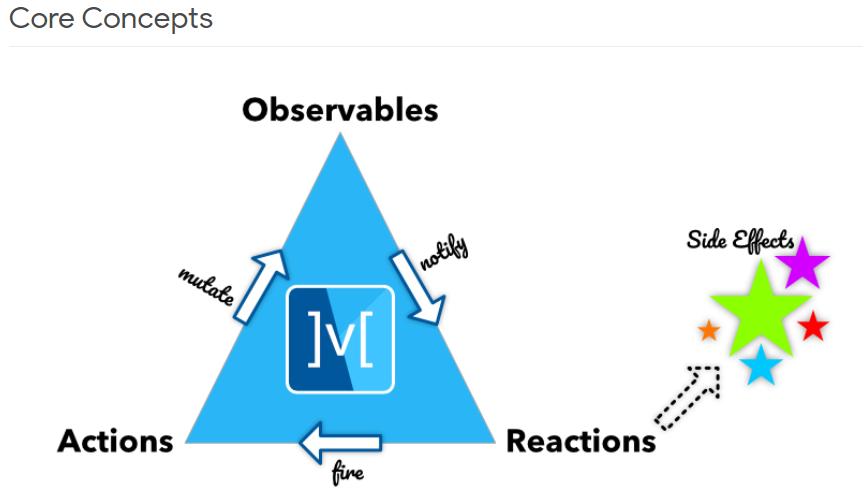
\includegraphics[height=7cm, width=12cm]{MobX.png}
\end{figure}
\\
\item We use Mobx together the concept of \textbf{Provider} in fact before running the app, we create a list of global providers. 
The Provider package allows us to inject our store and retrieve them anywhere from our widget tree.
\item We decided to use \textbf{Firebase Cloud Storage API} that let us to upload  users' data to firebase cloud and download it. It is a flexible and scalable NoSql database for mobile development. We protect the data for users logged in our app throght the use of certain rules with firebase authentication. Security, of course, is our first concern. All transfers are performed over a secure connection.
Firebase SDKs for Cloud Storage add Google security to file uploads and downloads for your Firebase apps, regardless of network quality. We use that SDKs to store images and other user-generated content like dishes and symptoms. 
Firebase Cloud is also use to share standard dishes and symptoms  between all logged users. We developers have to mantain them updated. 
In order to integrate firebase into our application we used FlutterFire that is a set of Flutter plugins which connect our Flutter application to Firebase:
\\
\begin{minipage}{0.3\linewidth}
    
\includegraphics[width=\linewidth]{FlutterAndFirebase.PNG}
\end{minipage}\hfil
\begin{minipage}{0.55\linewidth}
\begin{itemize}[•]
\item cloud\textunderscore firestore: 0.14.1+3
\item firebase\textunderscore storage: 5.1.0
\item firebase\textunderscore core: 0.5.0
\item firebase\textunderscore auth: 0.18.3
\end{itemize}
\end{minipage}

To handle the authentication of external services (google, github and twitter) we also imported the firebase plugin: lit\textunderscore firebase\textunderscore auth: 0.3.0 
\\

\item We have also integrated  \textbf{Open Food Facts} which is a database of food products with ingredients, allergens, nutritional information and all the details of information that can be found on product labels.
We used Flutter package for the Open Food Facts API. It can let us to Easily access to more than 1.5 million products from all around the world. Open Food Facts is powered by global contributors and is constantly growing thanks to them.
The user of our application can scan the barcode of a food and thanks to the integration of our system with Open Food Facts database we can show him/her the ingredients.
\begin{figure}[ht!]
\centering

\includegraphics[height=7cm, width=8cm]{openfoodfacts.png}
\end{figure}

\end{itemize}


\subsection{Software System Attributes} 

\subsubsection{Usability}
The age range of the users of our application is between 14 and 60 years old.
Our software is designed to be as simple as possible with 4 main pages where there is all the information at your fingertips and few actions that can be performed on them.\\
We have tried to make the insertion of the dishes fast and intuitive without the need to specify too precise times but only through 4 main moments of the meals.
We have chosen only 8 symptoms to avoid too much dispersion in the choice and visualization of data.\\
The symptoms chosen are the most common and related to the foods eaten.
Also the insertion of symptoms consists in selecting only 3 values already pre-set without having to type anything.\\
The graphs represent concepts simple to understand but at the same time very useful to the user such as the symptom that appears most often.
\subsubsection{Reliability}
The system is designed to be always reliable, using an online database managed by google we are always aware if our information has been saved or received correctly 24 hours a day.

\subsubsection{Availability}
The system, as far as the main information is concerned, guarantees a continuous and always available service by relying on Firebase as a remote server, which is managed by Google.\\
Although the availability offered by Open Food Fact is lower, this does not preclude the use of the main functions of the application.

\subsubsection{Security}
Users credentials and external services account will be cryptate and stored in Firebasewhich uses a hashing system to save passwords and thus make them secure.

\subsubsection{Maintainability}
The maintenance of the application is divided into three parts.
The first one is about data management, in particular periodically updating the default dishes we offer to users and adding some new symptoms if we notice that a large portion of users require them.\\
The second part is about improving the algorithm we use to process user data to offer more and more accurate and reliable statistics.\\
The third part is about keeping the application up to date with the various operating systems on which it runs (Android and iOS), while the part about databases and external systems is not our competition.
\subsubsection{Portability}
Our application offers a very high portability having leveraged Flutter as a programming platform that offers the possibility to easily develop for Android, iOS and Web.
The data, having divided from the logic of presentation,  are easily shared by any platform a user wants to access them.
\section{Specific Requirement}
\subsection{User characteristics}
The main actor that interact with the system is the \textbf{Registered User} of the application.\\
The registered user can access to all the function of the application, and can link external available services to his account in the login page.\\
The application is designed for all those users who suffer from eating problems or chronic disorders in their daily diet and who experience frequent symptoms. The application would help them monitor the chronic pattern of symptoms and identify a correlation between what they eat and the symptoms they experience so that they can follow a food diet that may alleviate their symptoms in some way. 
\subsection{User Interface Design}
\
\begin{description}[leftmargin=1cm,rightmargin=1cm]
\item [  1)Home page]
\
\
\
\begin{figure}[h!]
\centering
\hspace*{\fill}
\begin{subfigure}[tl]{0.3\linewidth}
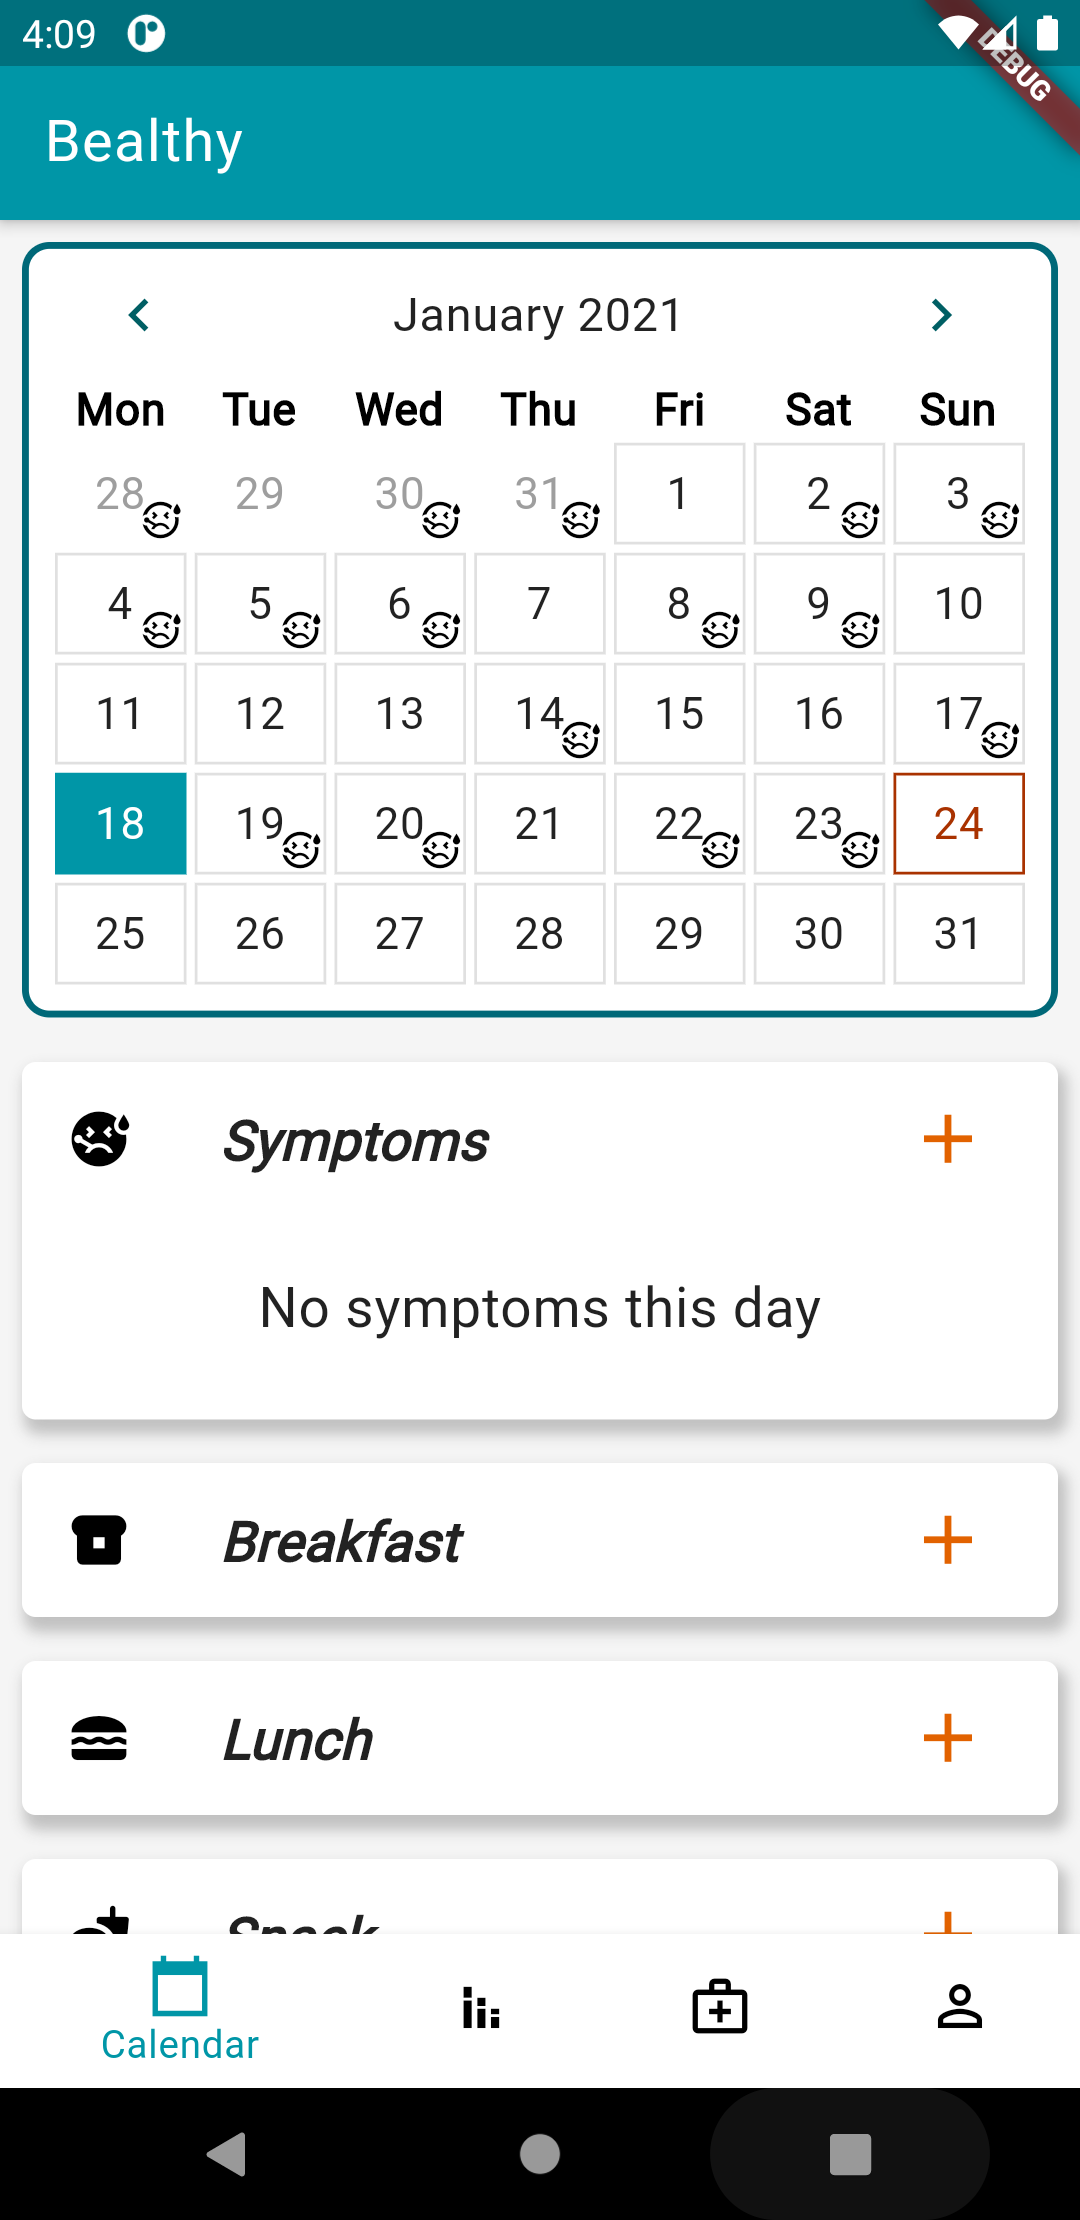
\includegraphics[width=\linewidth]{HomePage1.PNG}
\caption{\textbf{Empty day}}
\end{subfigure}\hfill
\begin{subfigure}[tr]{0.3\linewidth}
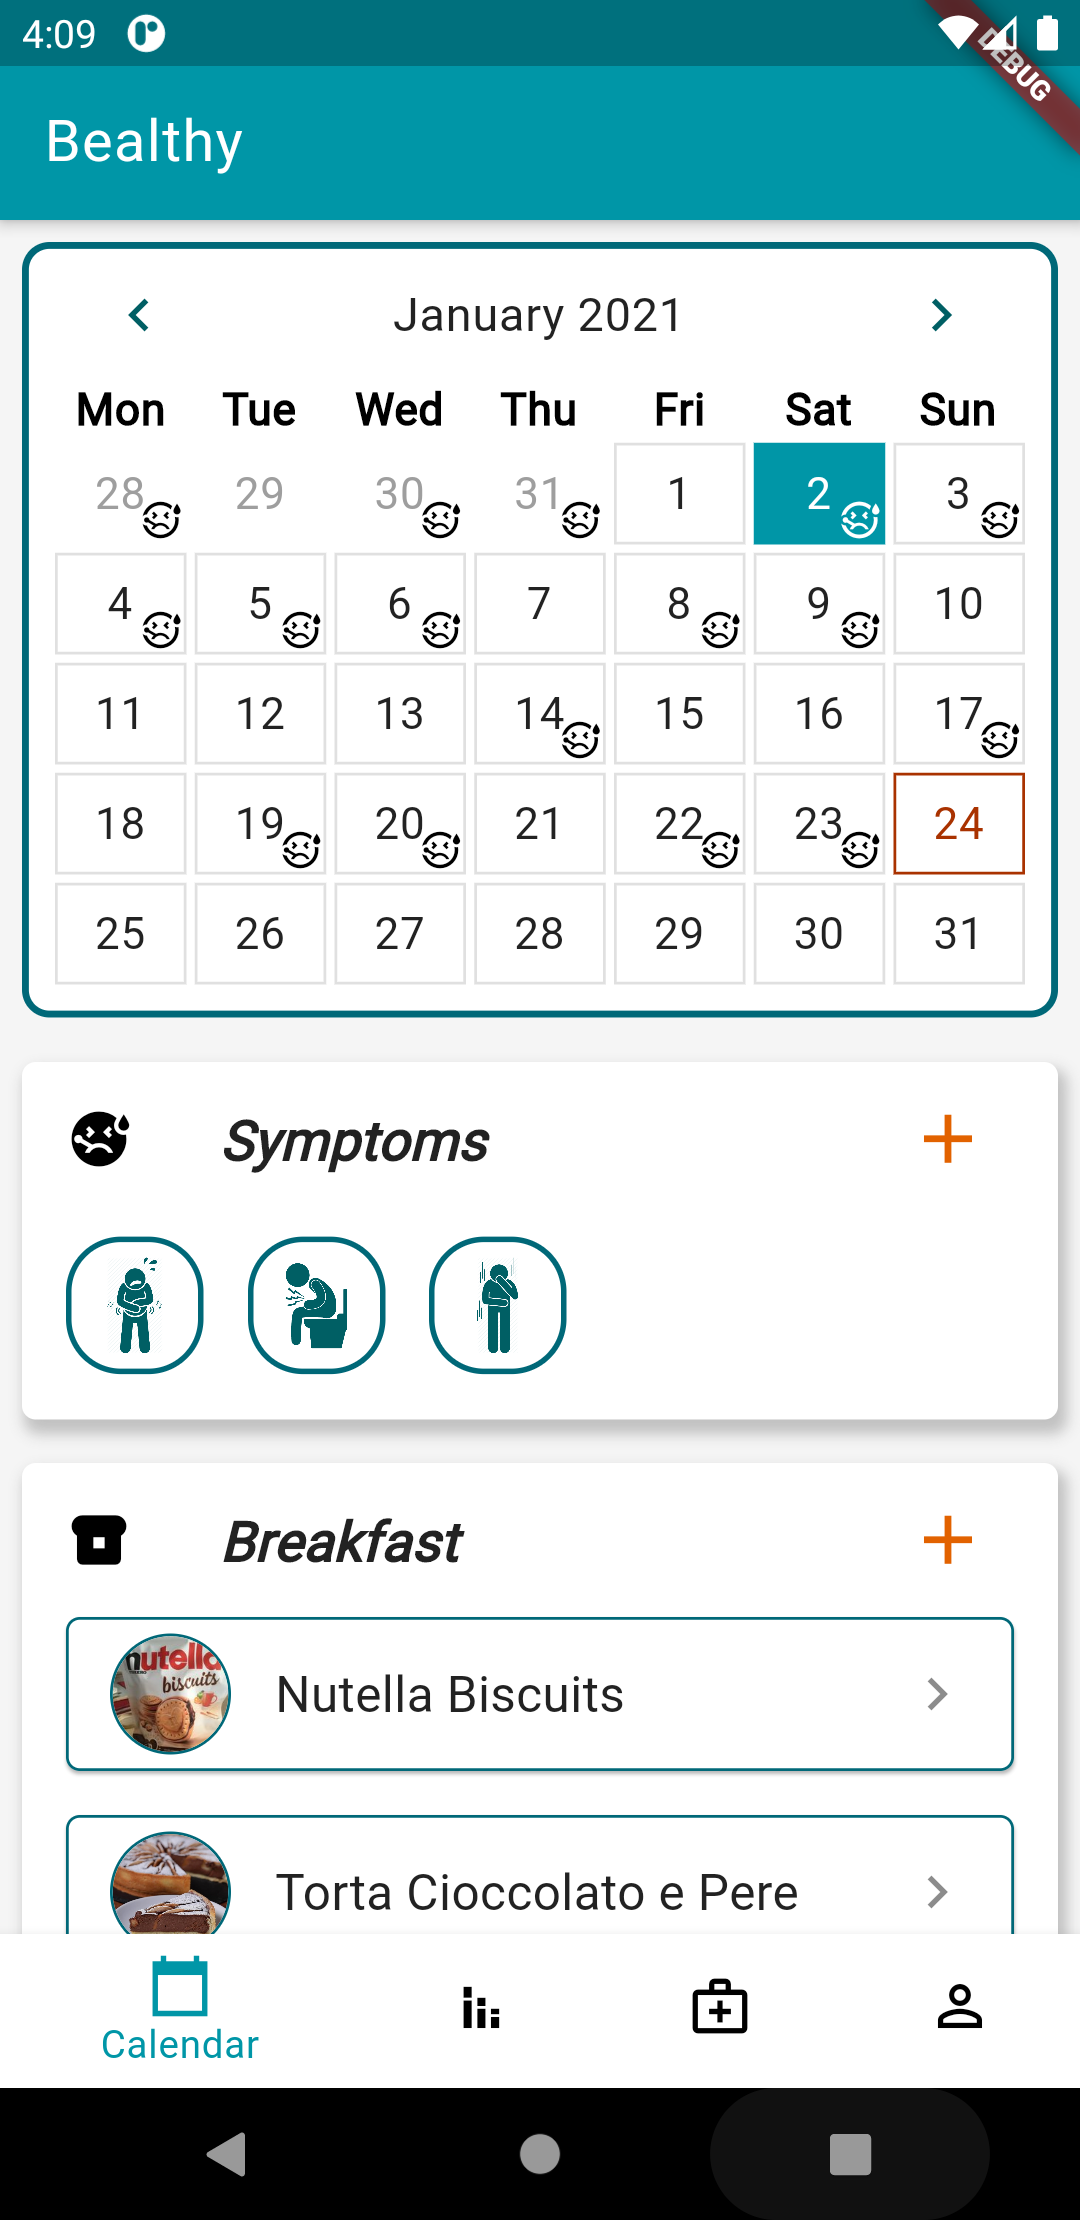
\includegraphics[width=\linewidth]{HomePage2.PNG}
\caption{\textbf{Day with symptoms and dishes}}
\end{subfigure}
\hspace*{\fill}
\end{figure}

\begin{itemize}[•]
\item This is the main screen of the application, from this screen the user can navigate through the calendar by simply clicking on any day. The side arrows allow the user to change the month selected on the calendar.  Underneath the calendar, the user can both view and keep track of his or her symptoms and meals taken in the past days and enter new ones using the appropriate buttons.  Scrolling upwards, the calendar is reduced to a simple bar showing the day selected by the user. Again, the user can use the side arrows to change the day. The calendar also shows with a specific icon the presence or absence of a symptom on a given day so that it is easy to see which days the user has been sickest.
\item With the "+" button in the symptoms box the user can add a symptom.
\item With the "+" button in the mealtime boxes ( breakfast,lunch,snach and dinner) the user can add a dish.
\item With the bottom bar  it will be possible to navigate through the various screens(calendar , statistics , treatments and personal page).
\end{itemize}
\item [ 2)Add symptom page]
\
\
\
\begin{figure}[h!]
\centering
\hspace*{\fill}
\begin{subfigure}[tl]{0.3\linewidth}
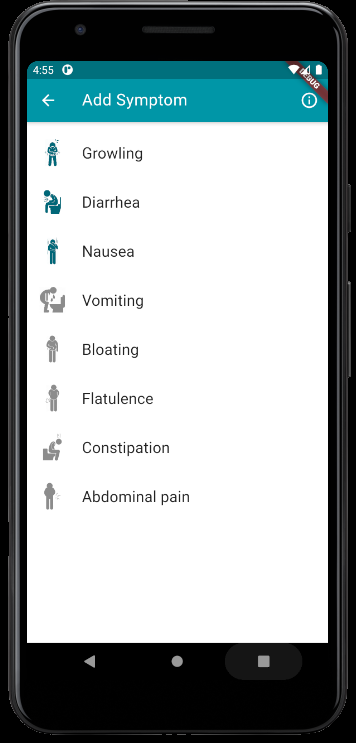
\includegraphics[width=\linewidth]{addSymptom1.PNG}
\caption{\textbf{All symptoms}}
\end{subfigure}\hfill
\begin{subfigure}[tr]{0.3\linewidth}
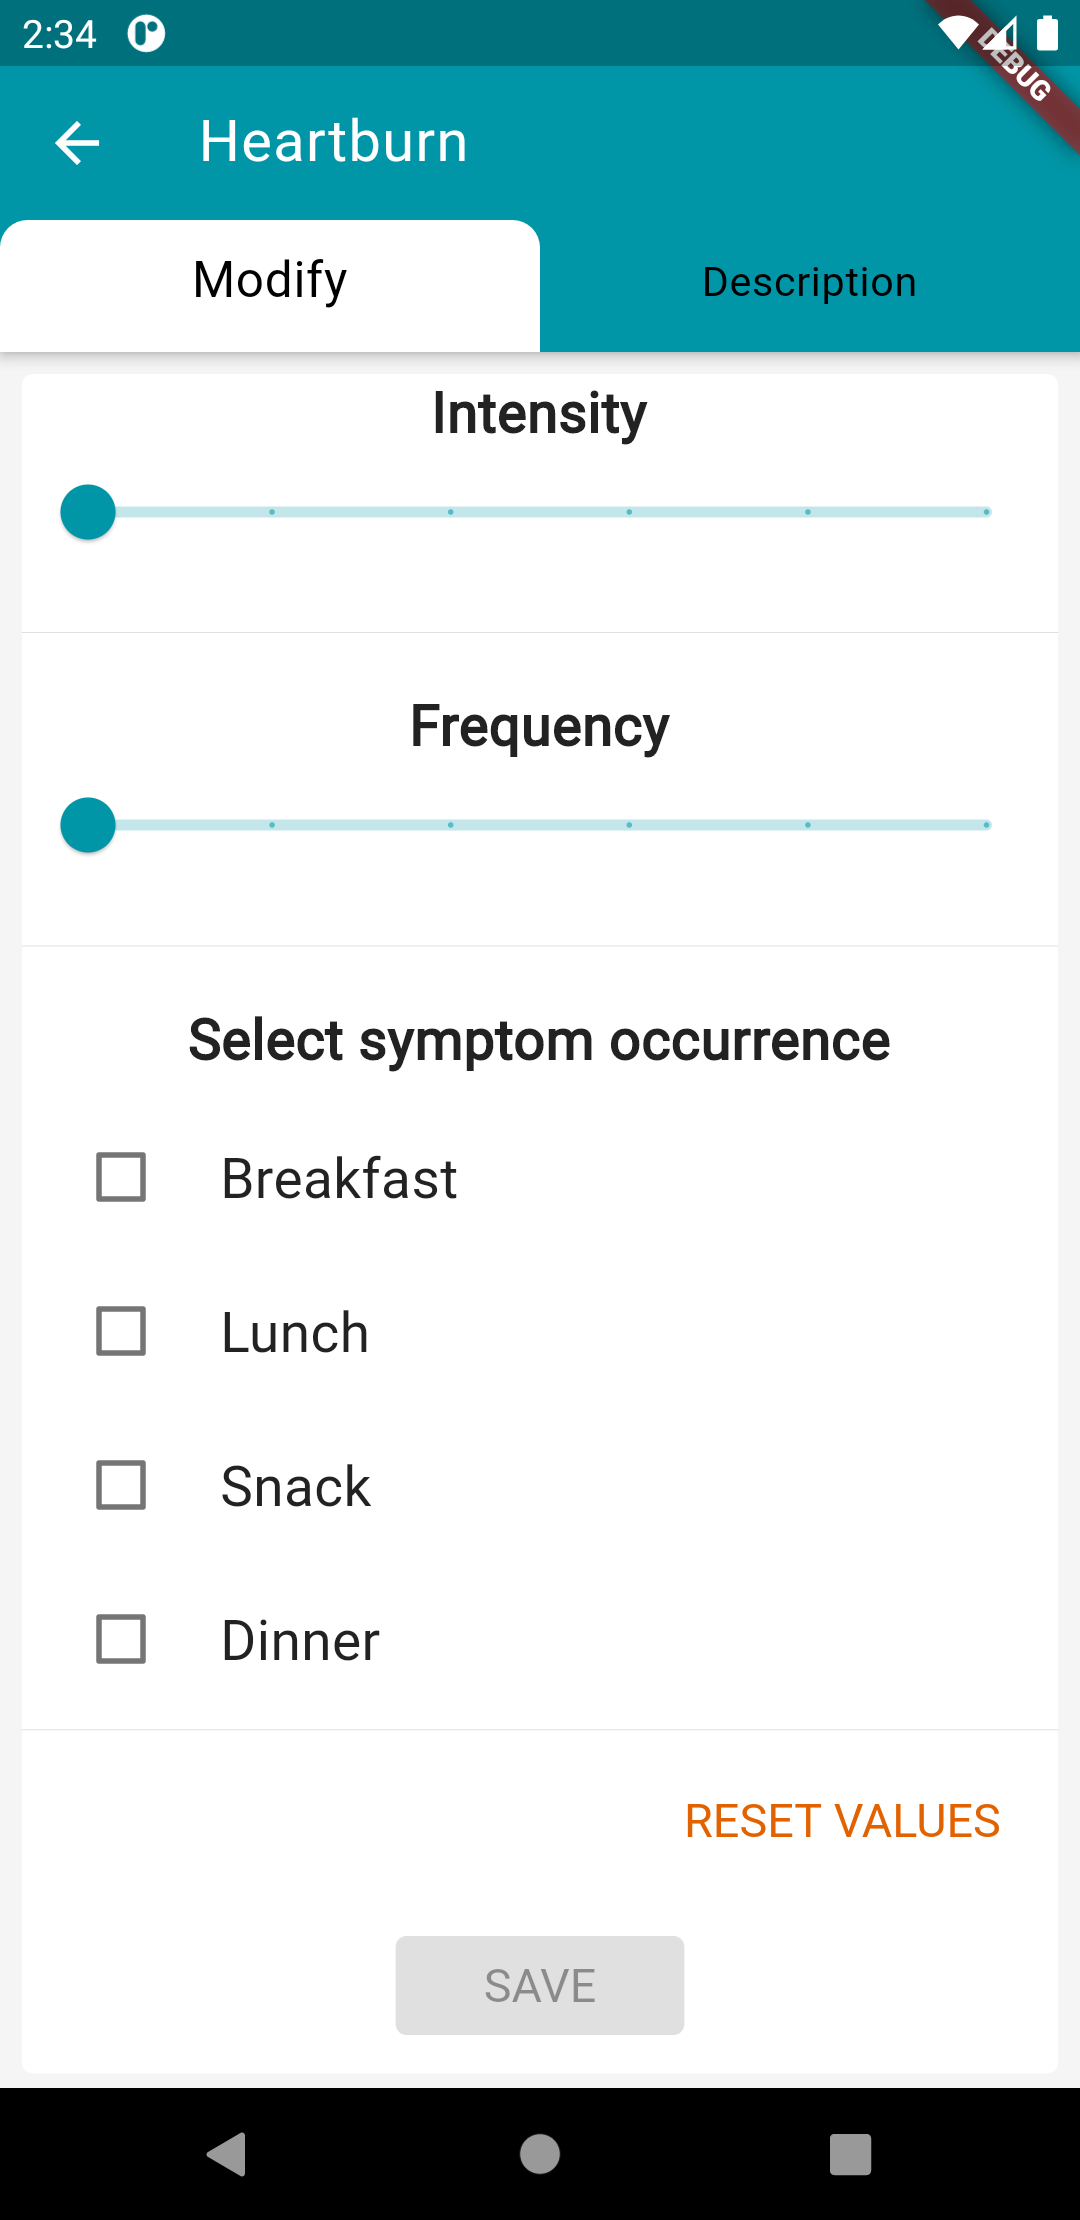
\includegraphics[width=\linewidth]{addSymptom2.PNG}
\caption{\textbf{Add symptom}}
\end{subfigure}
\hspace*{\fill}
\begin{subfigure}[tr]{0.3\linewidth}
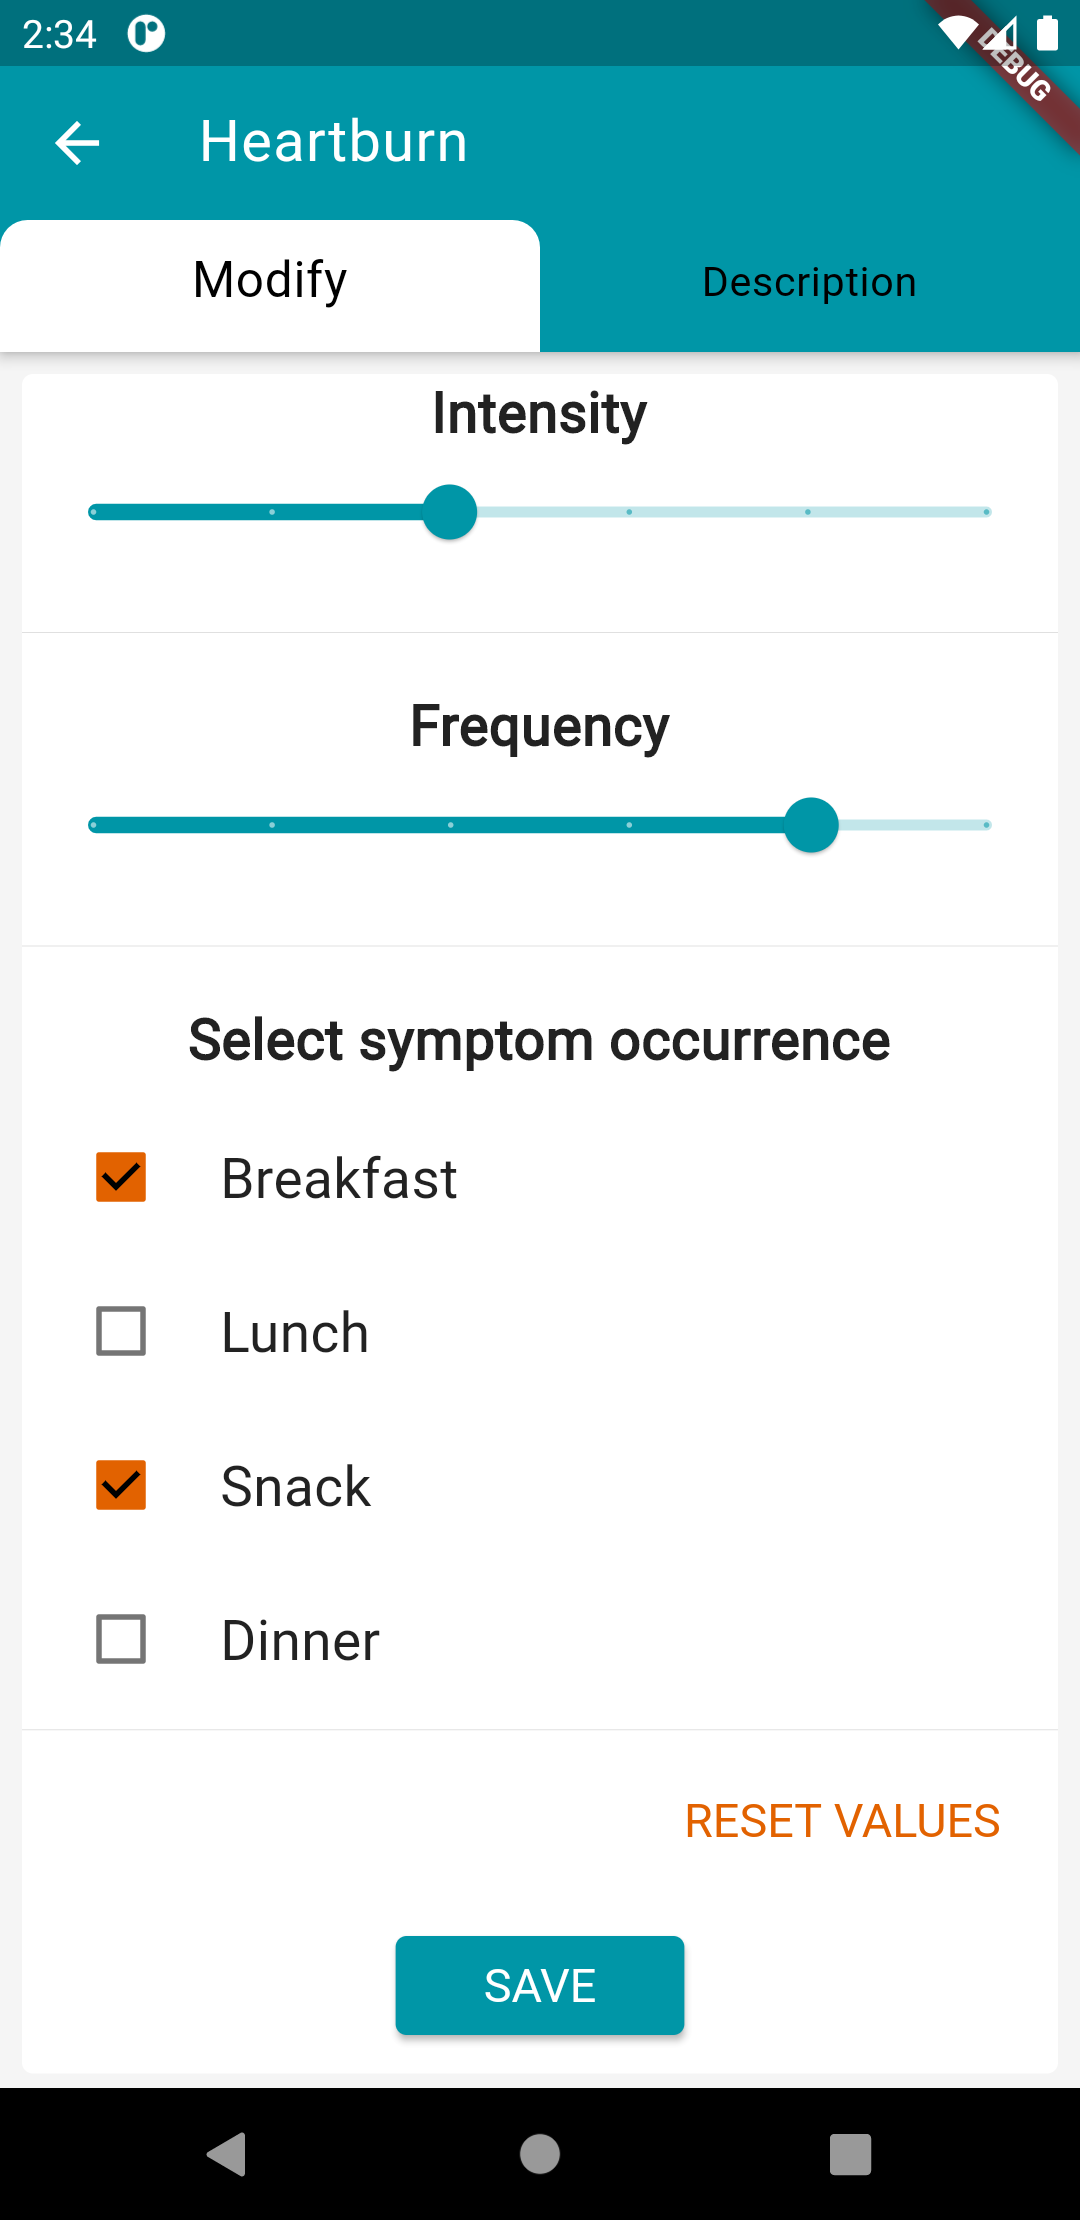
\includegraphics[width=\linewidth]{addSymptom3.PNG}
\caption{\textbf{Set parameters}}
\end{subfigure}
\hspace*{\fill}
\end{figure}
\begin{itemize}[•]
\item The first picture shows the all symptoms screen that is displayed after clicking on the "+" button in the symptom box under the calendar in the Homepage screen. 
\item After clicking on a specific symptom, a form will appear. The second picture shows this form that the user needs to complete in order to be able to add a new symptom in the selected day. 
\item It's necessary set all the parameters: intensity, frequency and when the symptom occurs in order to click on the "save" button.
\end{itemize}
\clearpage
\item [ 3)Add Dish page]
\
\
\
\begin{figure}[h!]
\centering
\hspace*{\fill}
\begin{subfigure}[tl]{0.3\linewidth}
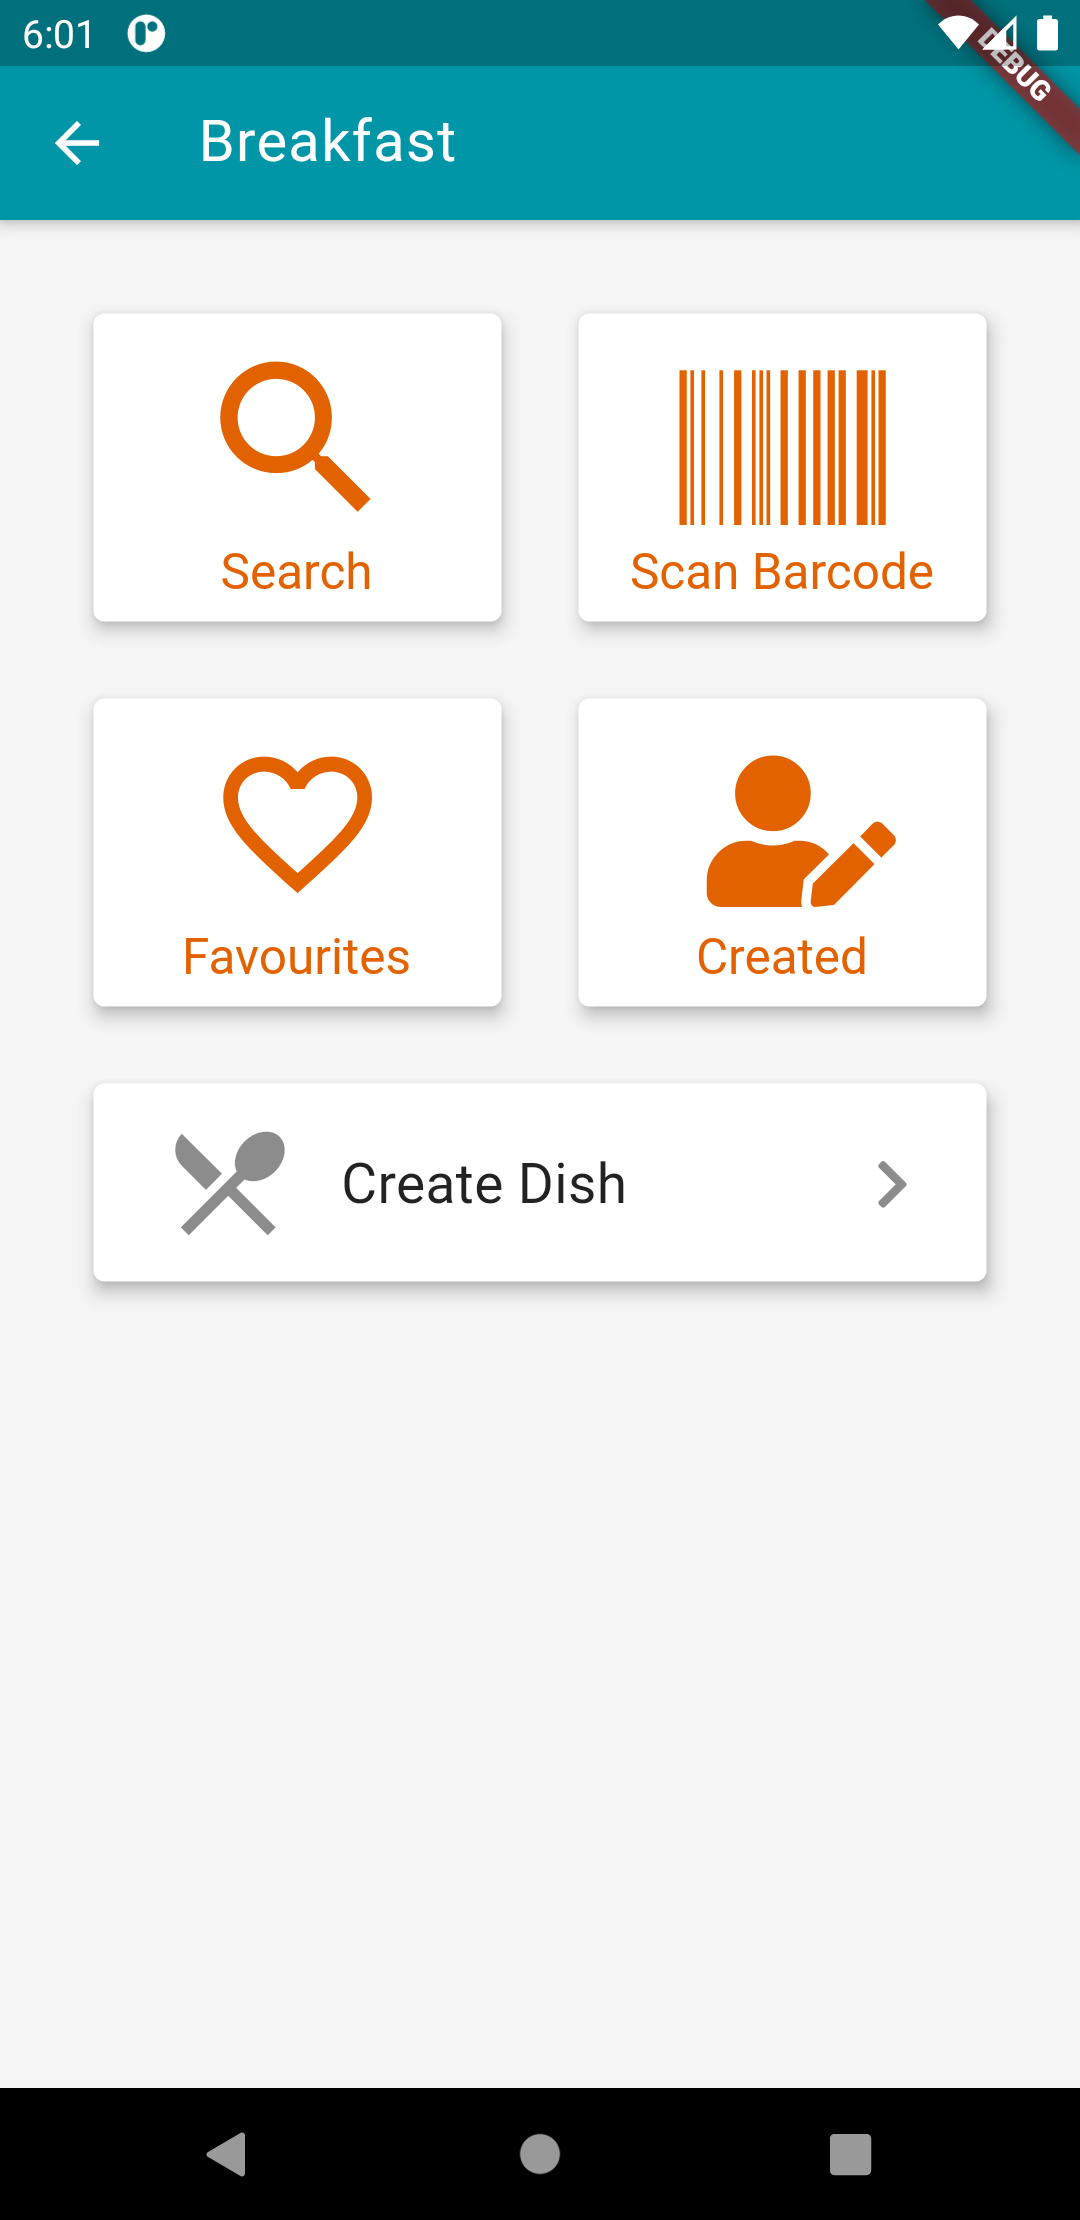
\includegraphics[width=\linewidth]{addDish1.PNG}
\caption{\textbf{Add dish}}
\end{subfigure}\hfill
\begin{subfigure}[tr]{0.3\linewidth}
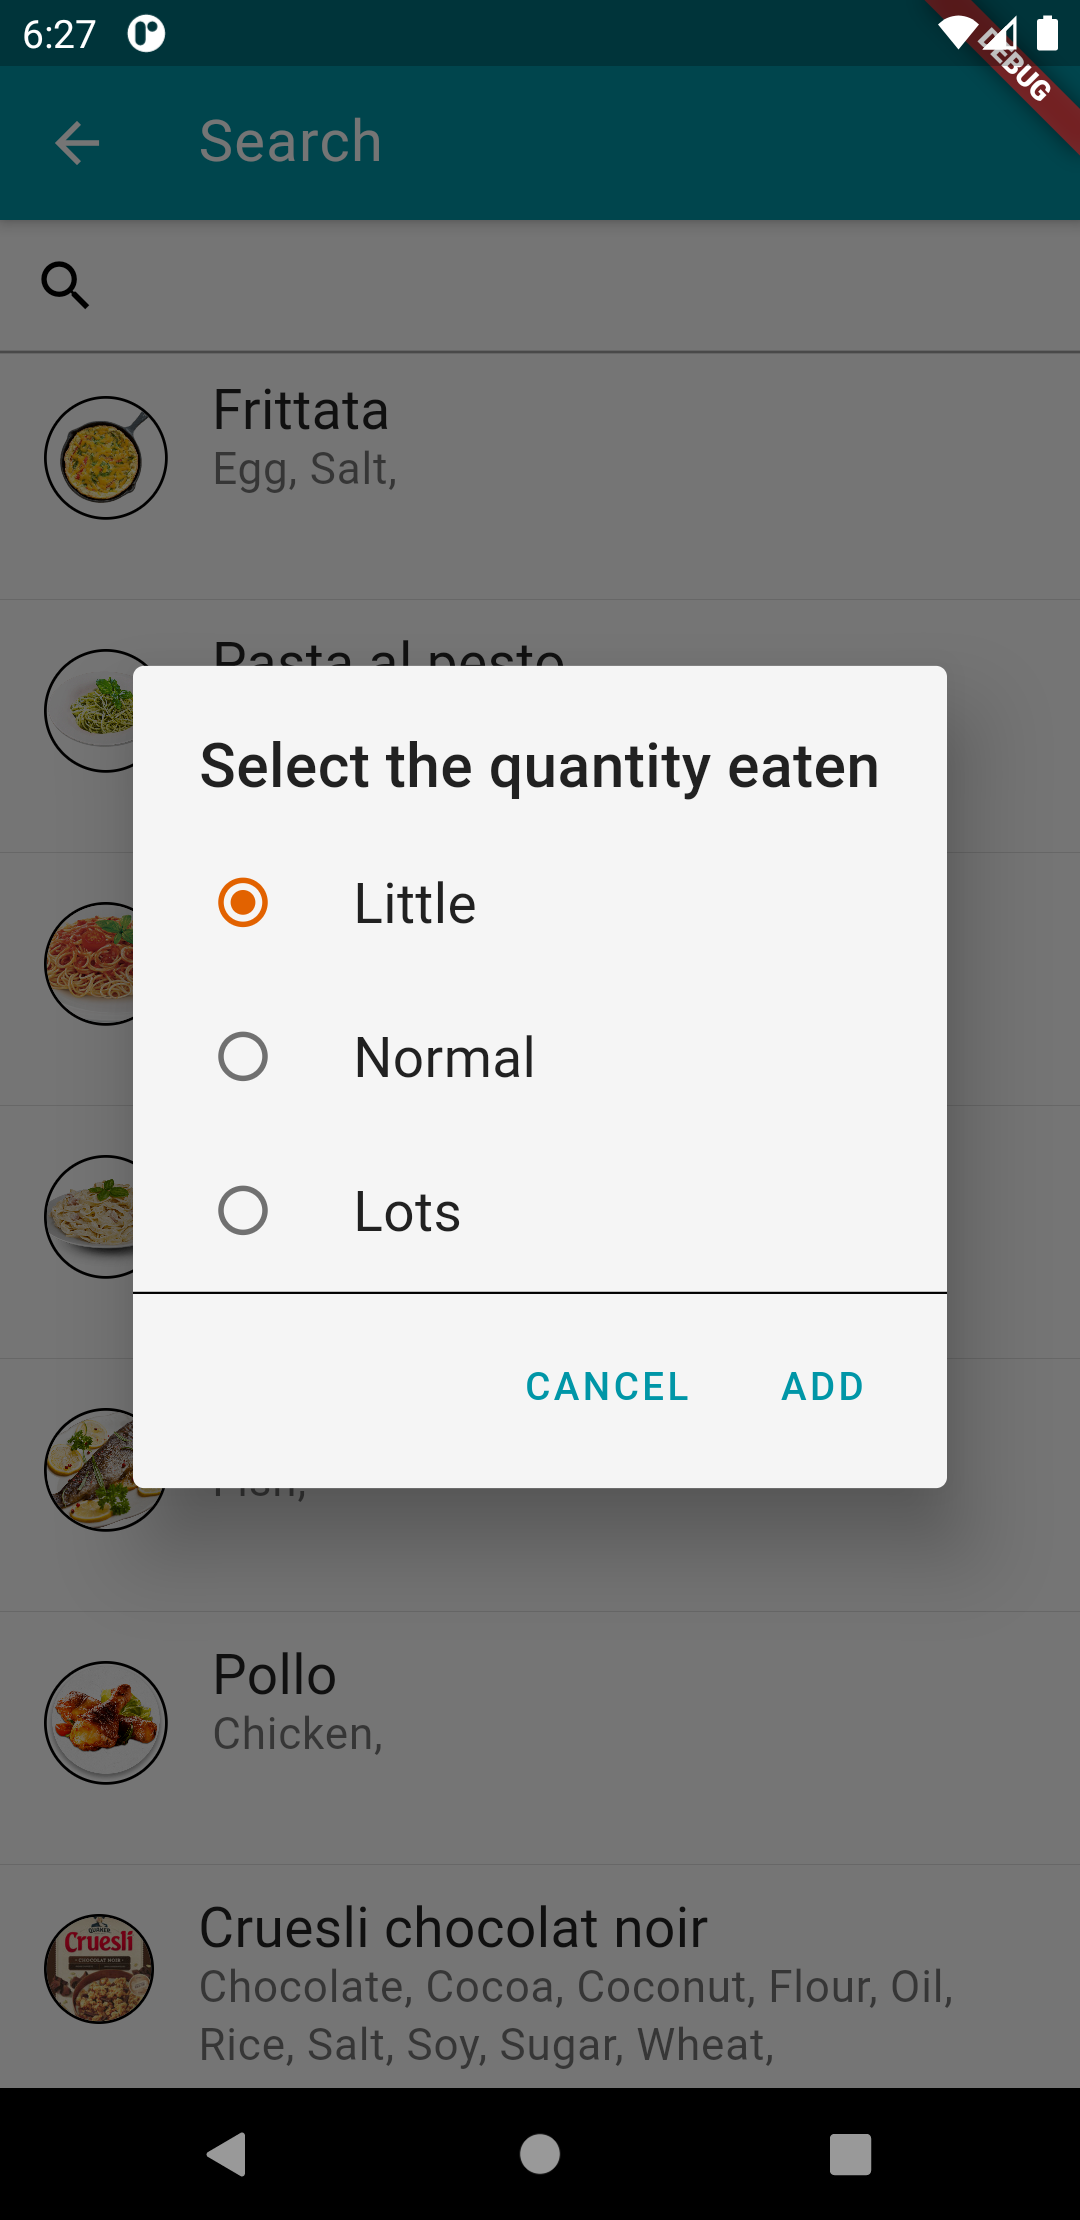
\includegraphics[width=\linewidth]{addDish5.PNG}
\caption{\textbf{Search Dishes}}
\end{subfigure}
\hspace*{\fill}
\begin{subfigure}[tr]{0.3\linewidth}
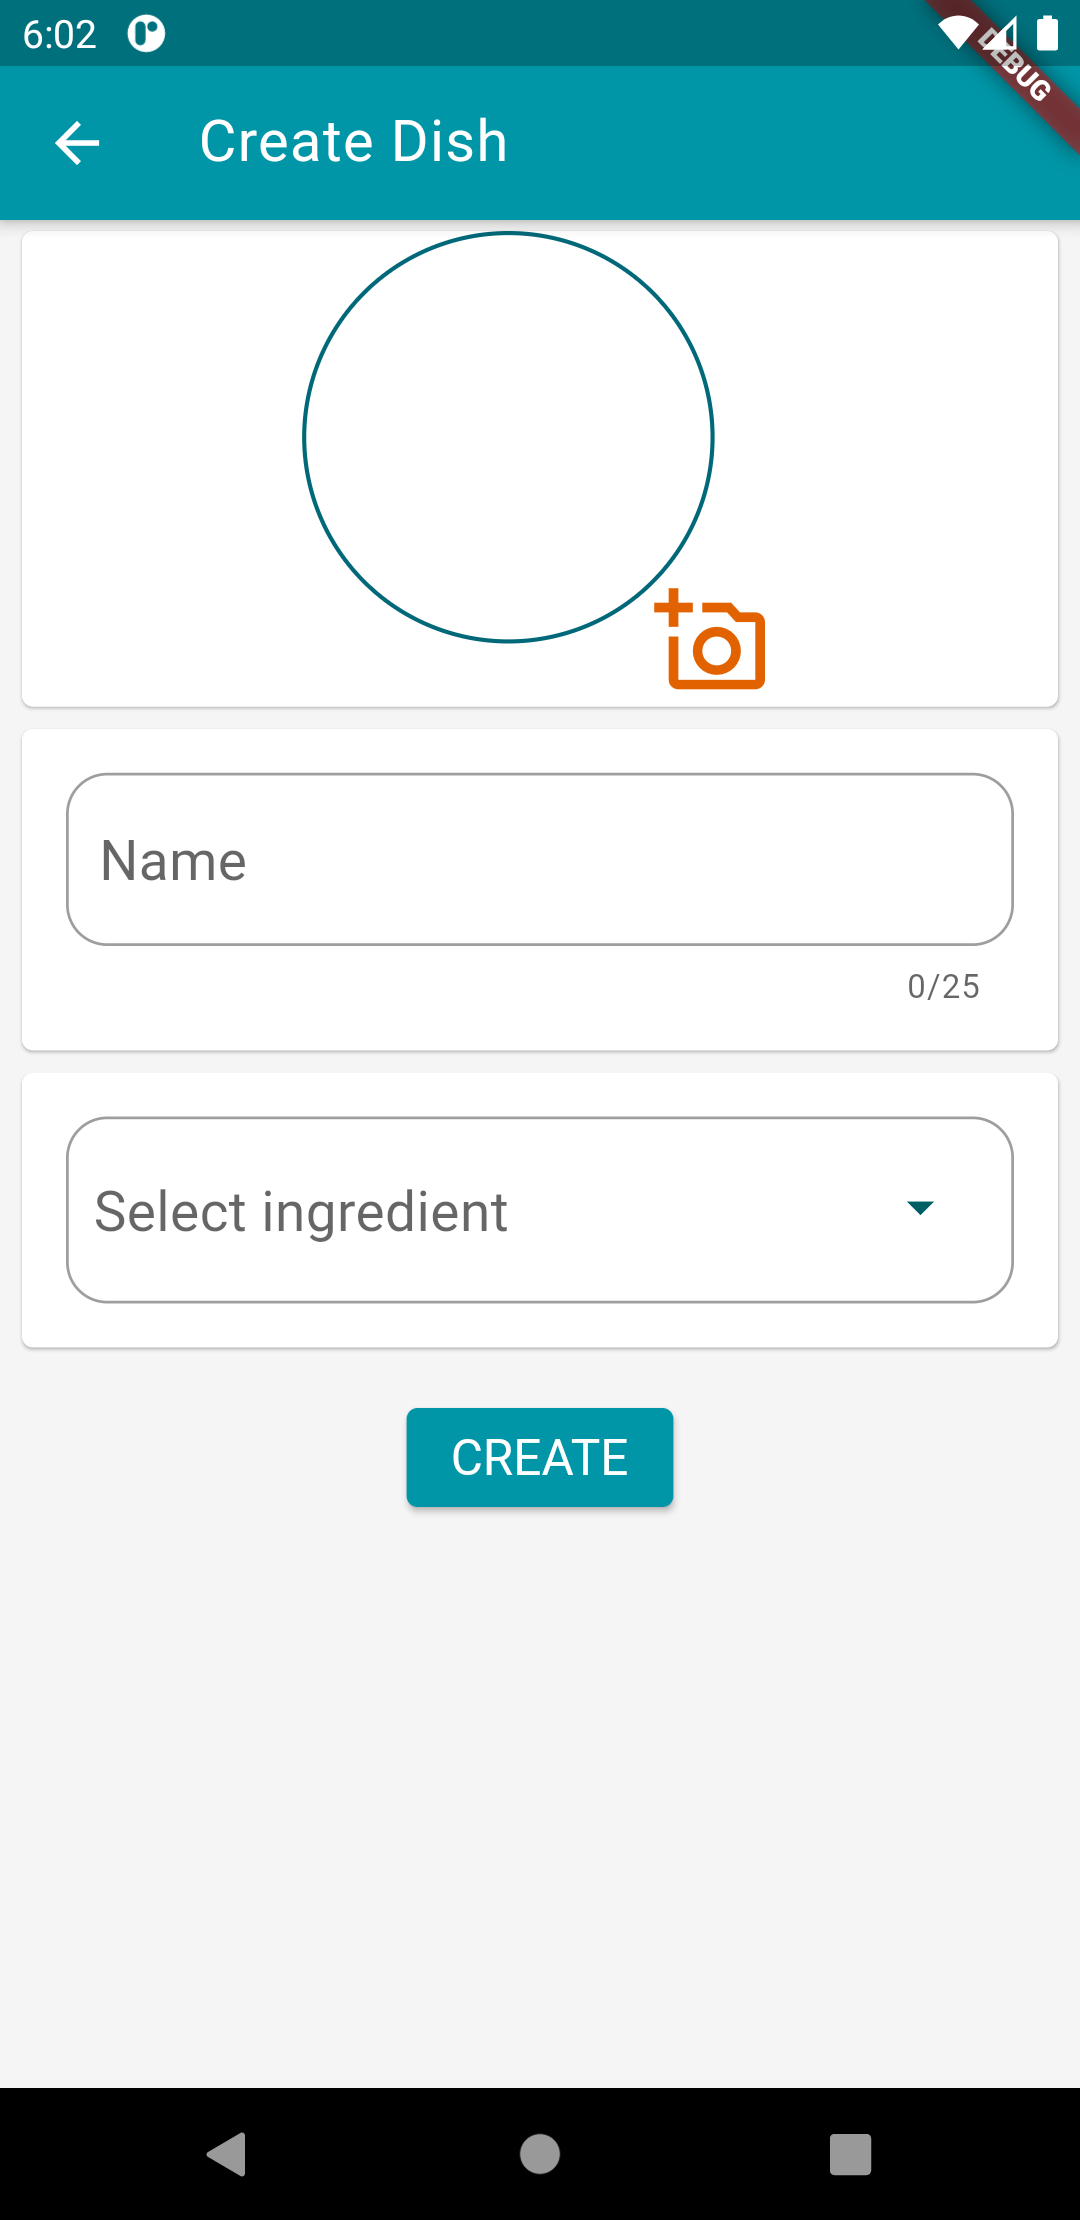
\includegraphics[width=\linewidth]{addDish2.PNG}
\caption{\textbf{Create dish}}
\end{subfigure}
\hspace*{\fill}
\begin{subfigure}[tr]{0.3\linewidth}
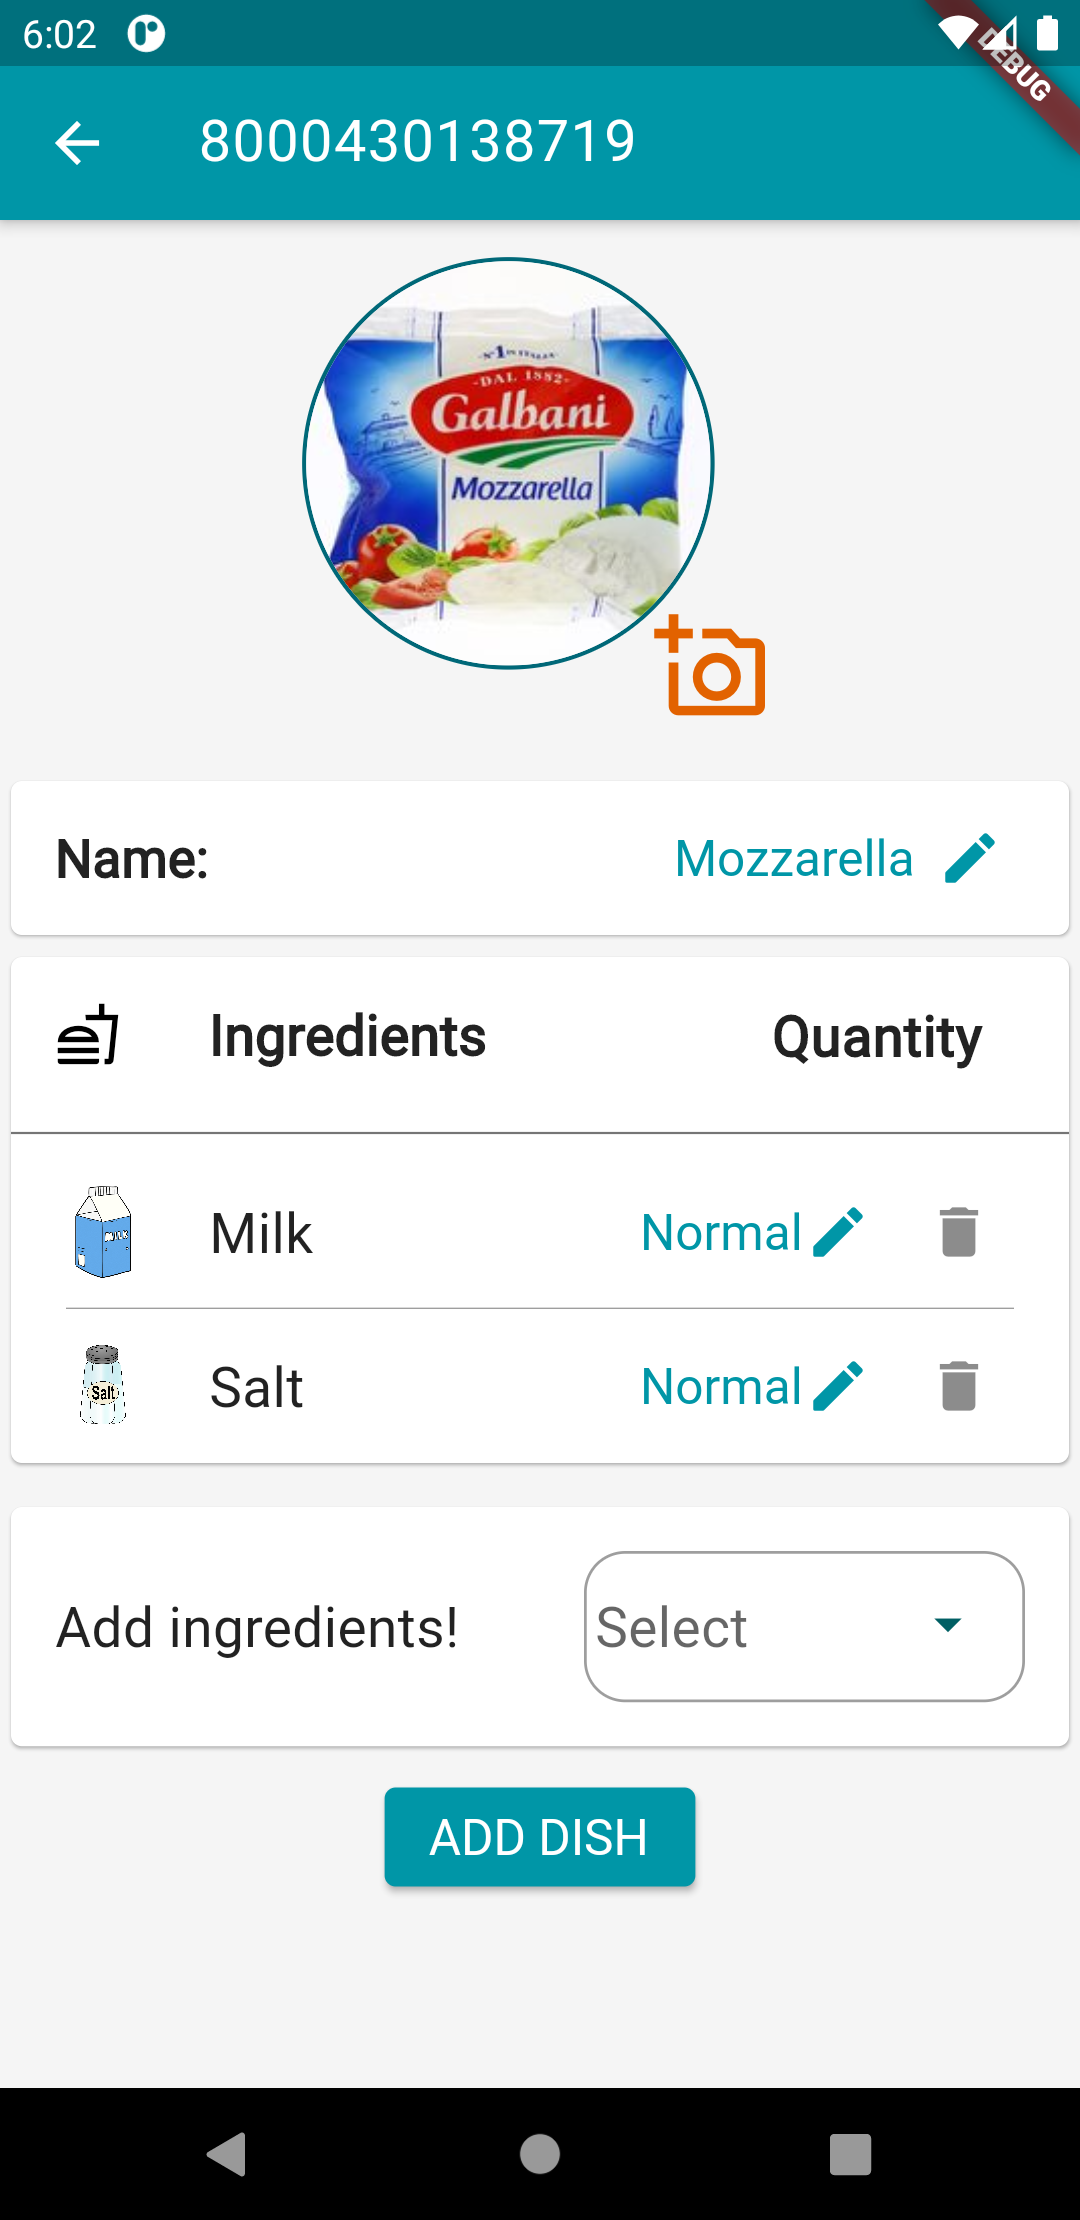
\includegraphics[width=\linewidth]{addDish3.PNG}
\caption{\textbf{Scanned dish}}
\end{subfigure}
\hspace*{\fill}
\end{figure}
\\
\begin{itemize}[•]
\item The first picture shows the five  ways to add a new dish in a specific mealtime of selected day. Three methods are similar and consists of a research of dish into a list(Search,favourite and created dishes buttons) the last two ones are two actions that the user can do. The user in fact can scan the barcode of a dish or can create a customizable dish inserting an image, a name, the list of ingredients and their quantity. 
\item The three searching ways are displayed with the same design. In each of them there is the list of dishes with which the user can interact. Clicking on one of the dishes, a popup will open that asks for the eaten quantity.
\item After clicking on "create" button, a form will appear. The picture shows this form that the user needs to complete in order to be able to add a new dish in the selected day.  This form let the user to customize a new dish with an image that can take with his/her camera or uploading an image from the  gallery, inserting a name and the list of ingredients.
\item The last picture shows the page of a dish scanned by the user with all the informations that have been collected by the Open Food Facts database. If the user wants, he/she can also insert other ingredients.
\end{itemize}

\item [ 4)Add treatment]
\
\
\
\begin{figure}[h!]
\centering
\hspace*{\fill}
\begin{subfigure}[tl]{0.3\linewidth}
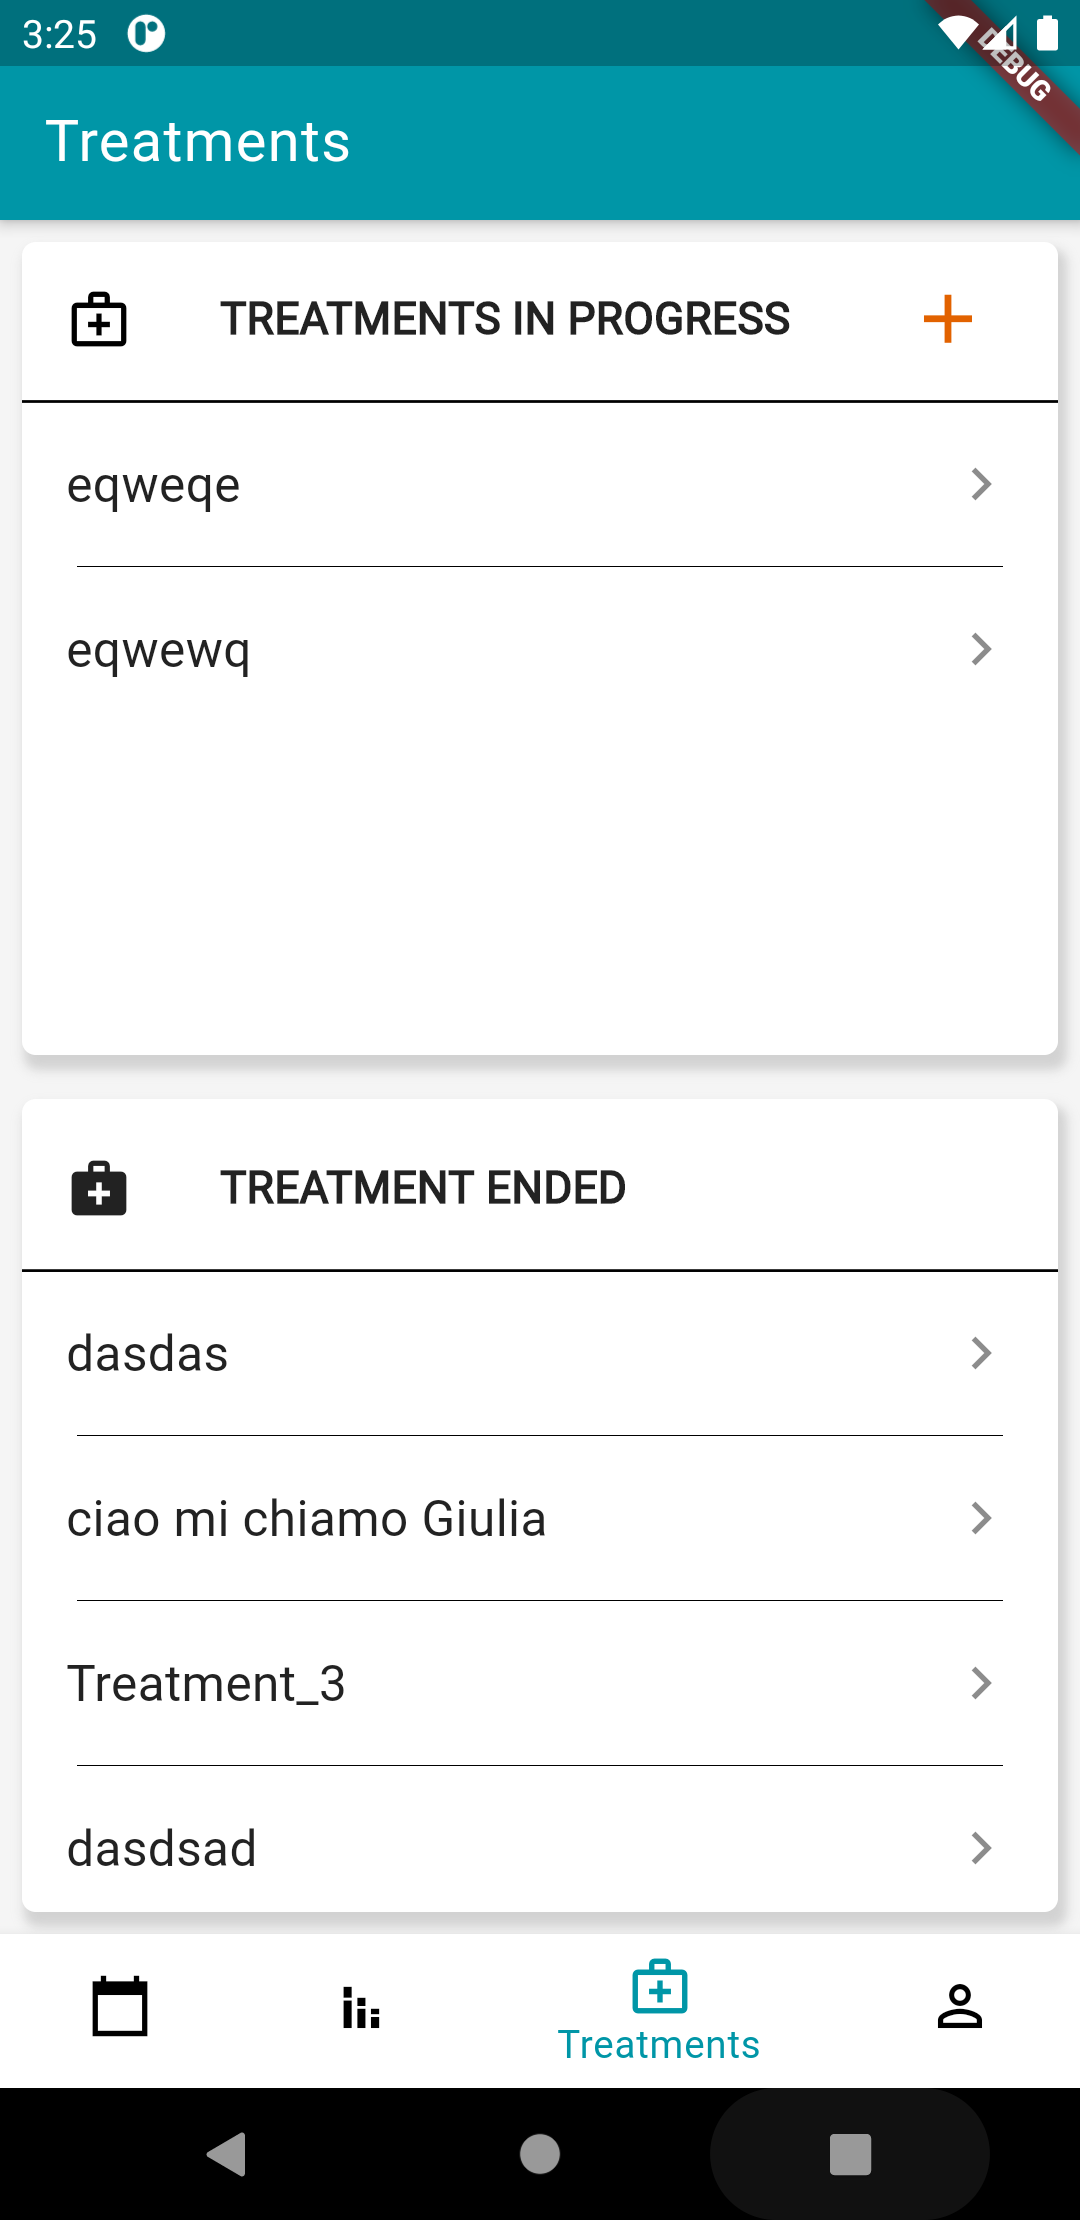
\includegraphics[width=\linewidth]{treatments1.PNG}
\caption{\textbf{Treatments}}
\end{subfigure}\hfill
\begin{subfigure}[tr]{0.3\linewidth}
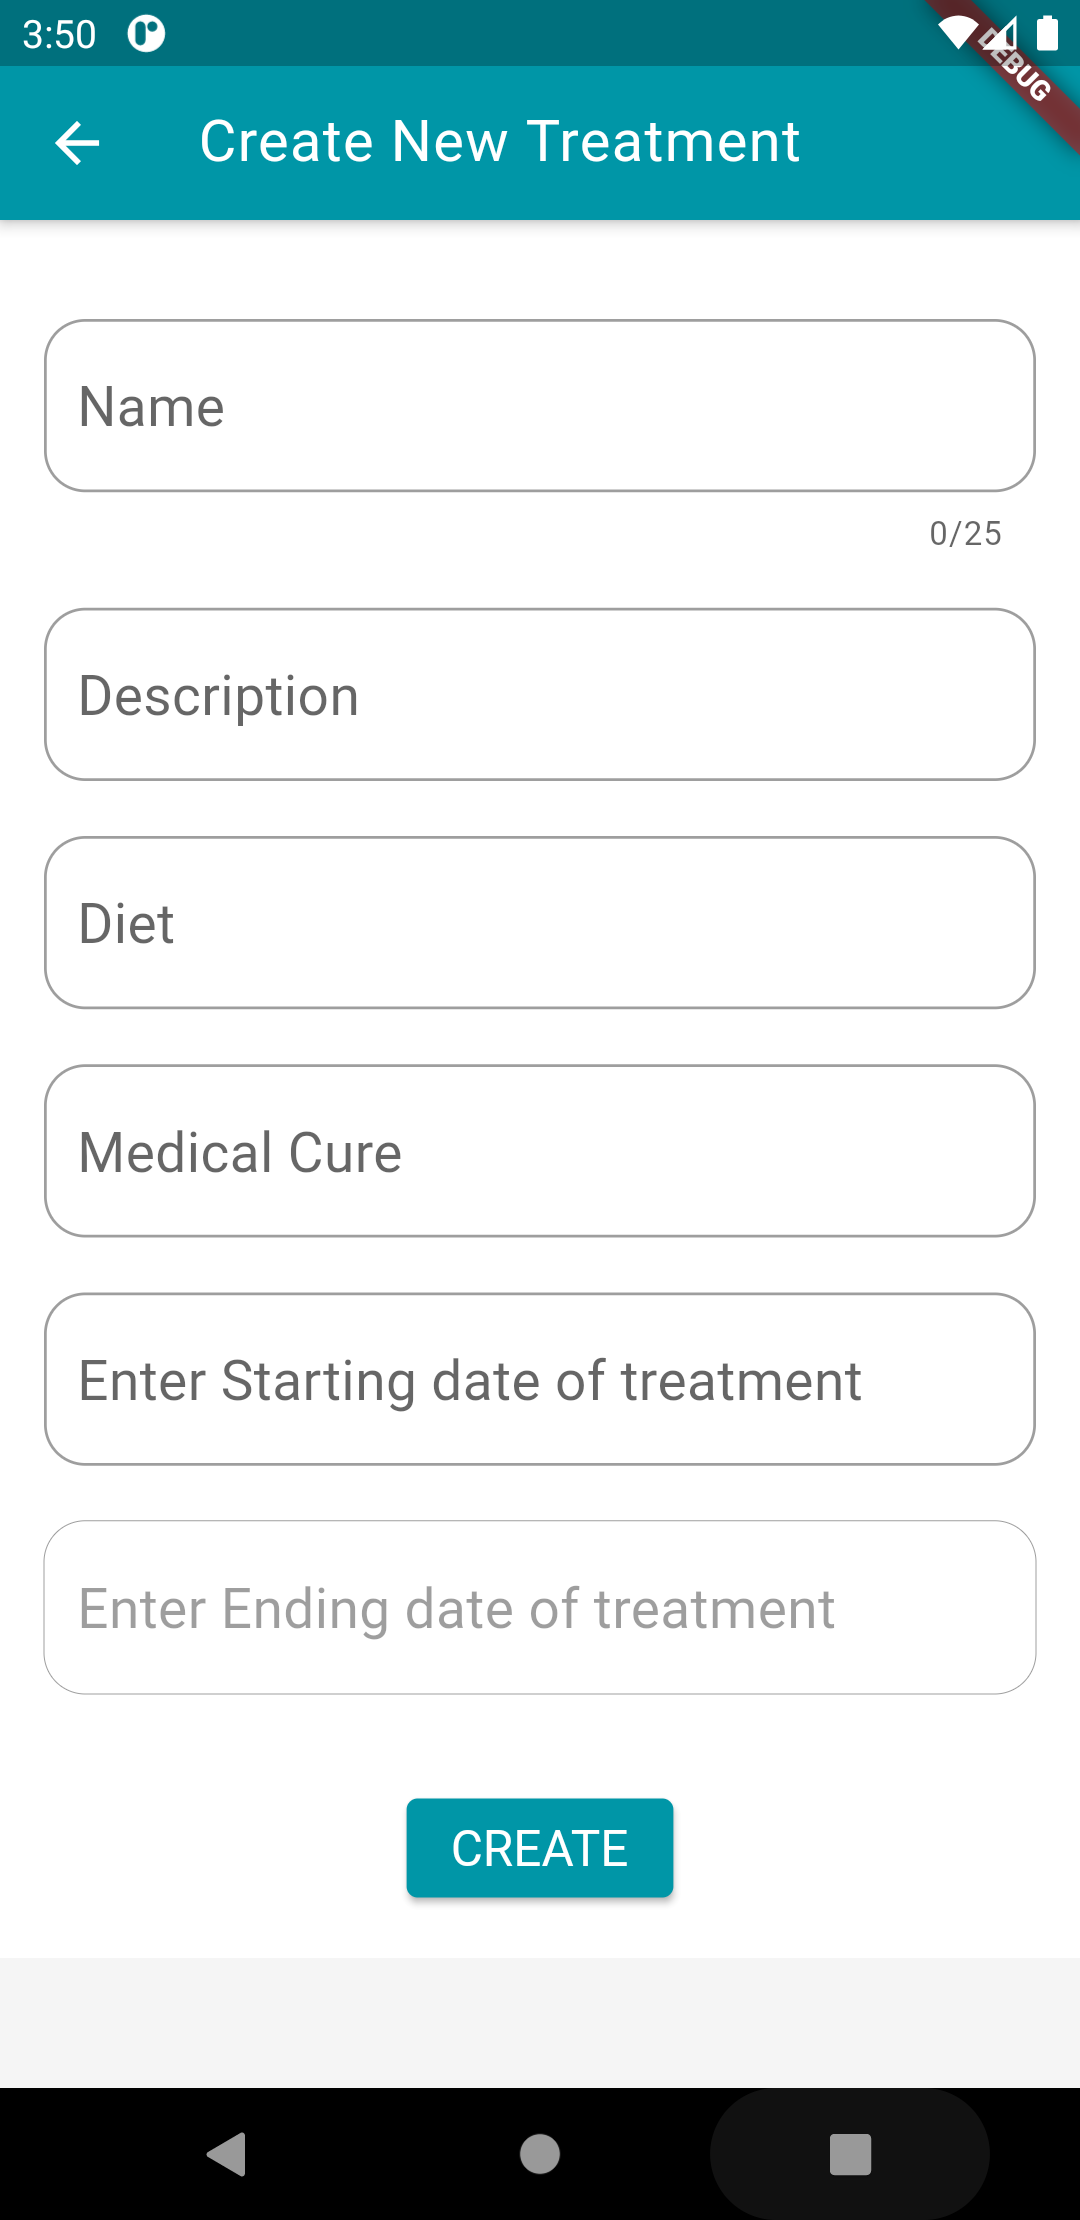
\includegraphics[width=\linewidth]{treatments4.PNG}
\caption{\textbf{Add treatment form}}
\end{subfigure}
\hspace*{\fill}
\end{figure}
\begin{itemize}[•]
\item The user can add a medical treatment or diet by clicking on the "+" button in the current treatments box. A form will open. The description, diet and medical cure are optional fields while everything else is compulsory as the dates are needed to show the user the percentage trend of symptoms before and after the end of these treatments. The user can then assess the effectiveness or otherwise of that particular treatment. 
\end{itemize}

\clearpage
\item [ 5)Visualize statistics]
\
\
\
\begin{figure}[h!]
\centering
\hspace*{\fill}
\begin{subfigure}[tl]{0.3\linewidth}
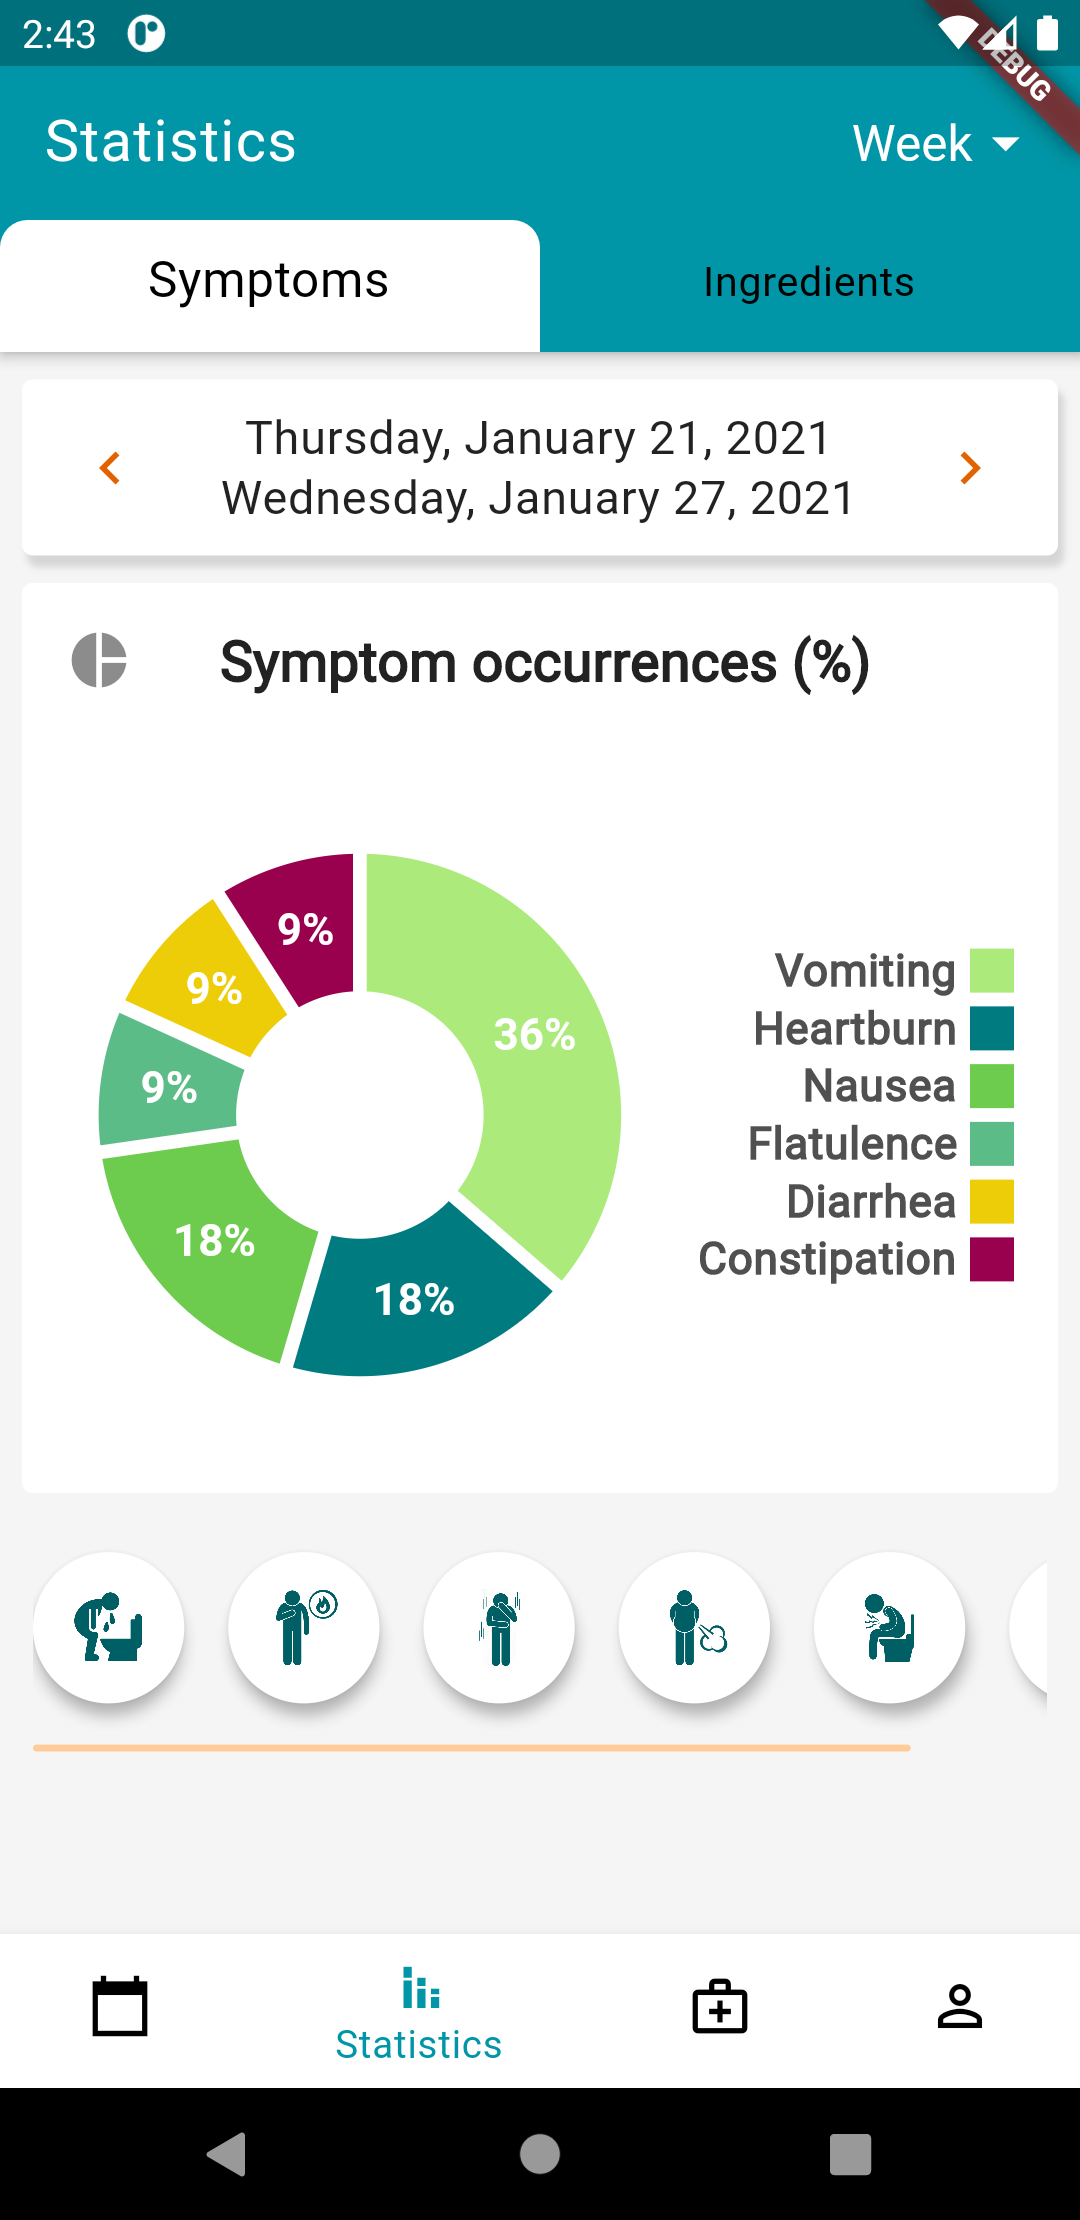
\includegraphics[width=\linewidth]{statistics1.PNG}
\caption{\textbf{Symptoms}}
\end{subfigure}\hfill
\begin{subfigure}[tr]{0.3\linewidth}
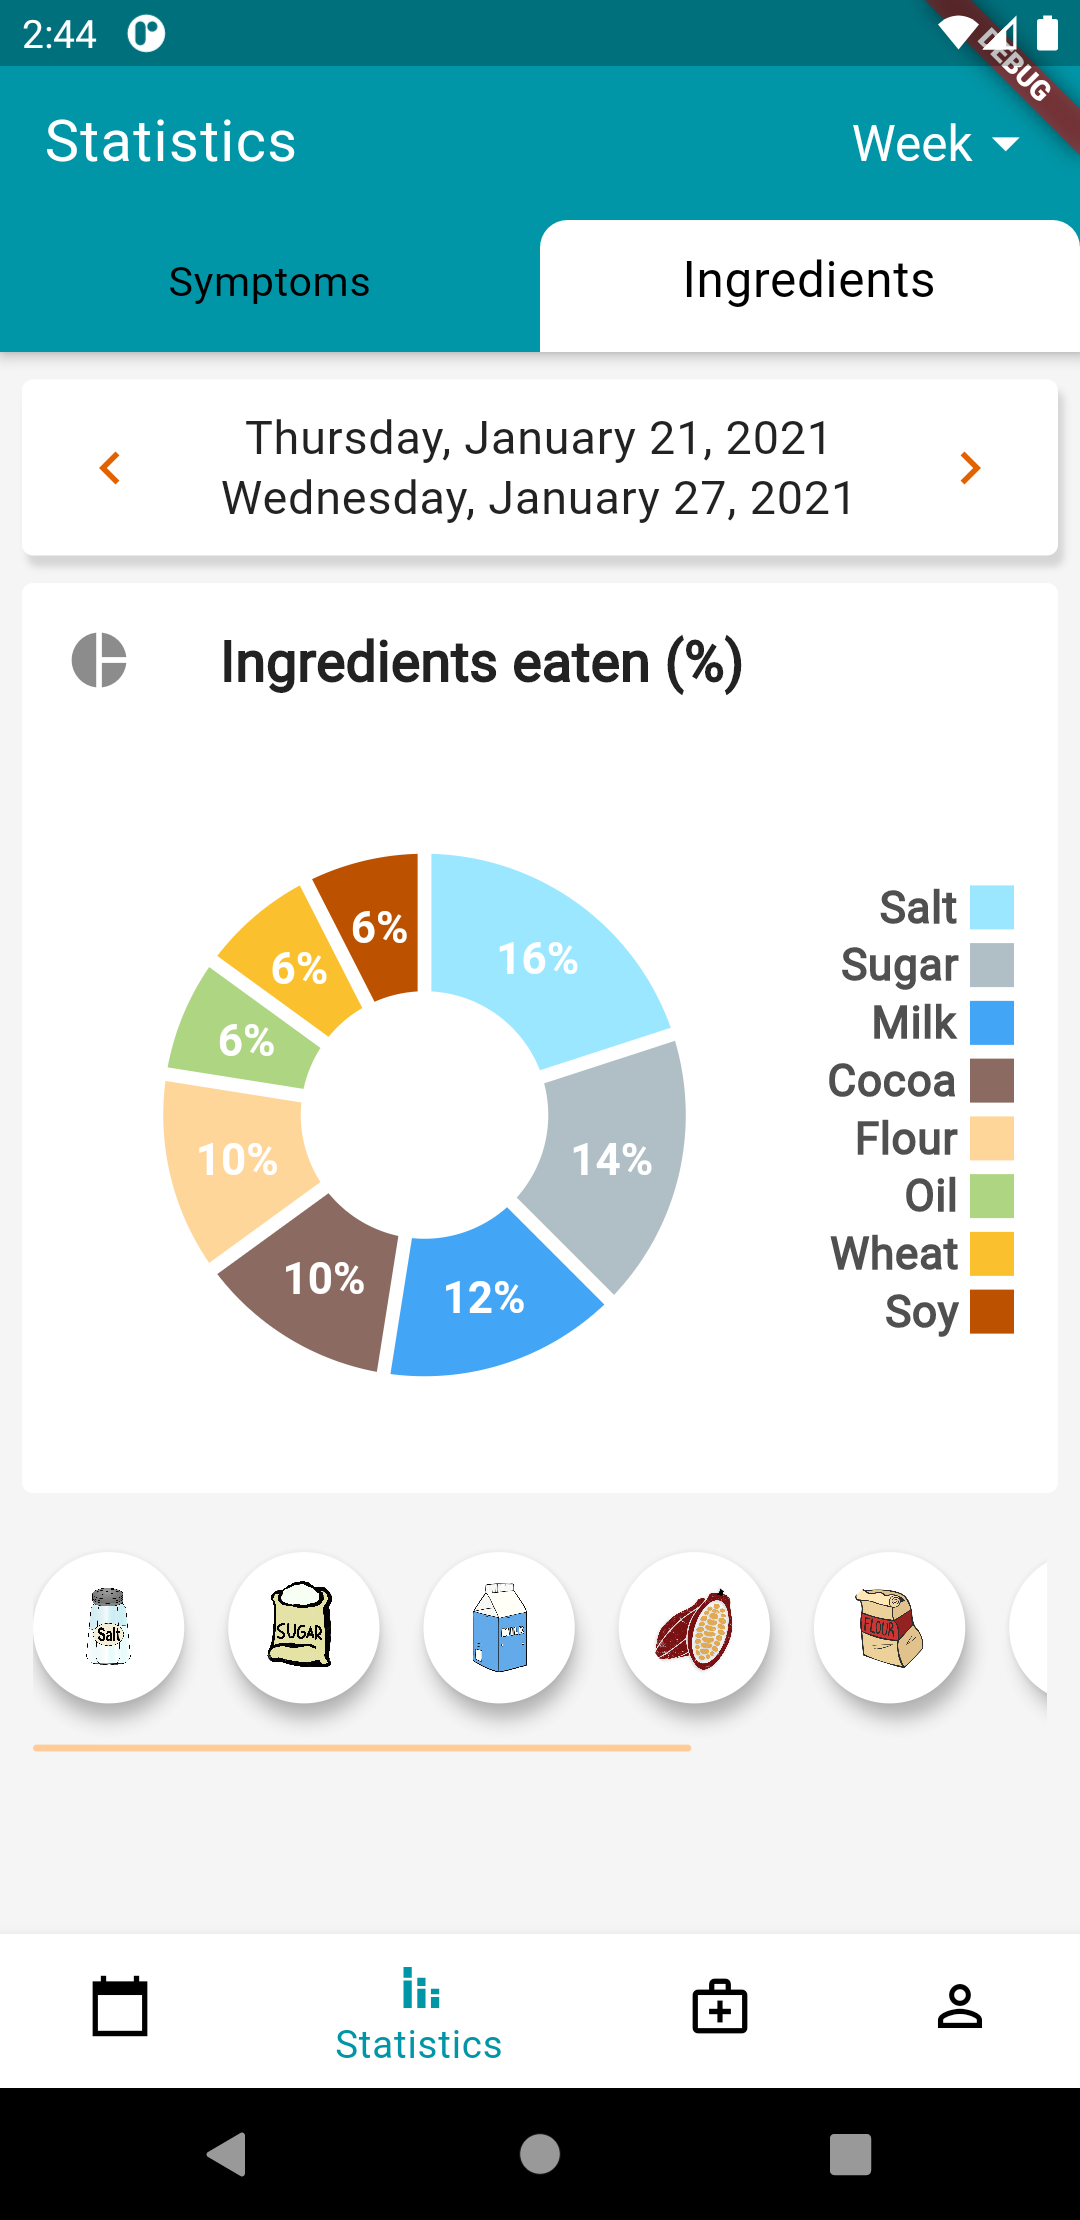
\includegraphics[width=\linewidth]{statistics2.PNG}
\caption{\textbf{Ingredients}}
\end{subfigure}
\hspace*{\fill}
\begin{subfigure}[tr]{0.3\linewidth}
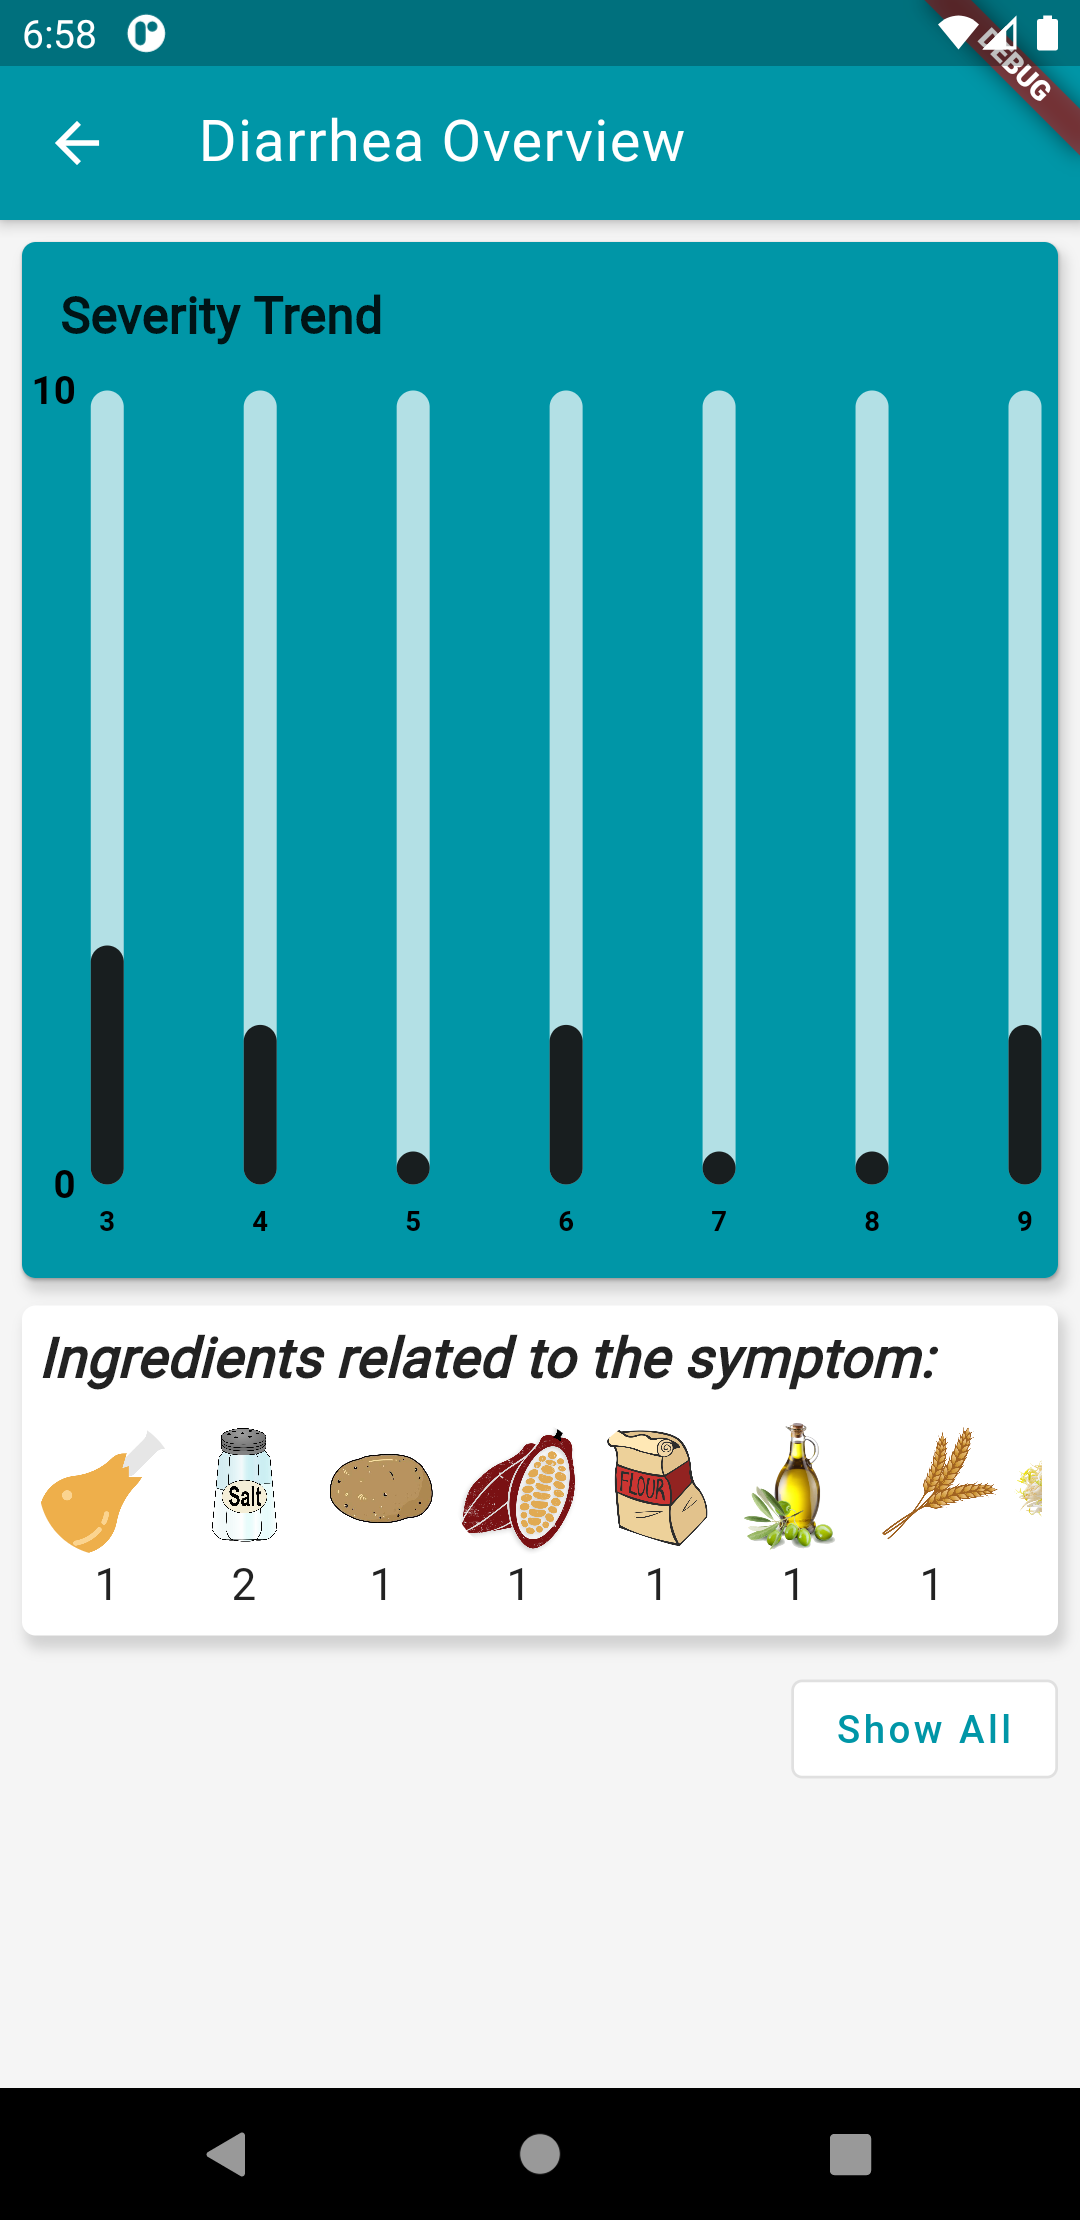
\includegraphics[width=\linewidth]{statistics3.PNG}
\caption{\textbf{Correlation between symptom and ingredients}}
\end{subfigure}
\hspace*{\fill}
\end{figure}
\begin{itemize}[•]
\item The statistics screen is divided into two tab bars: the first one shows the graph of the percentages of the symptoms and the second one that of the ingredients. The user can change the period for which the percentages are displayed using the menu at the top right. He can choose between week, month or set a date period through the use of a calendar. To change the week or month, he/she can use the side arrows under the tab bar while to change the date range, simply click on the calendar icon.
The symptom graph shows the user the percentages with which a symptom occurred in that time period. The ingredient graph shows the percentage of an ingredient eaten by the user.
\item By clicking on a specific symptom, below the pie chart with all the percentages, another bar chart will open showing the correlation between this symptom and the ingredients consumed by the user in the selected time period. The height of the bars indicates the value of the severity of the symptom on that day. If the user clicks on any day, the ingredients and their occurrences will be displayed below the graph.
\end{itemize}

\item [ 6)Visualize treatments]
\
\
\
\begin{figure}[h!]
\centering
\hspace*{\fill}
\begin{subfigure}[tl]{0.3\linewidth}
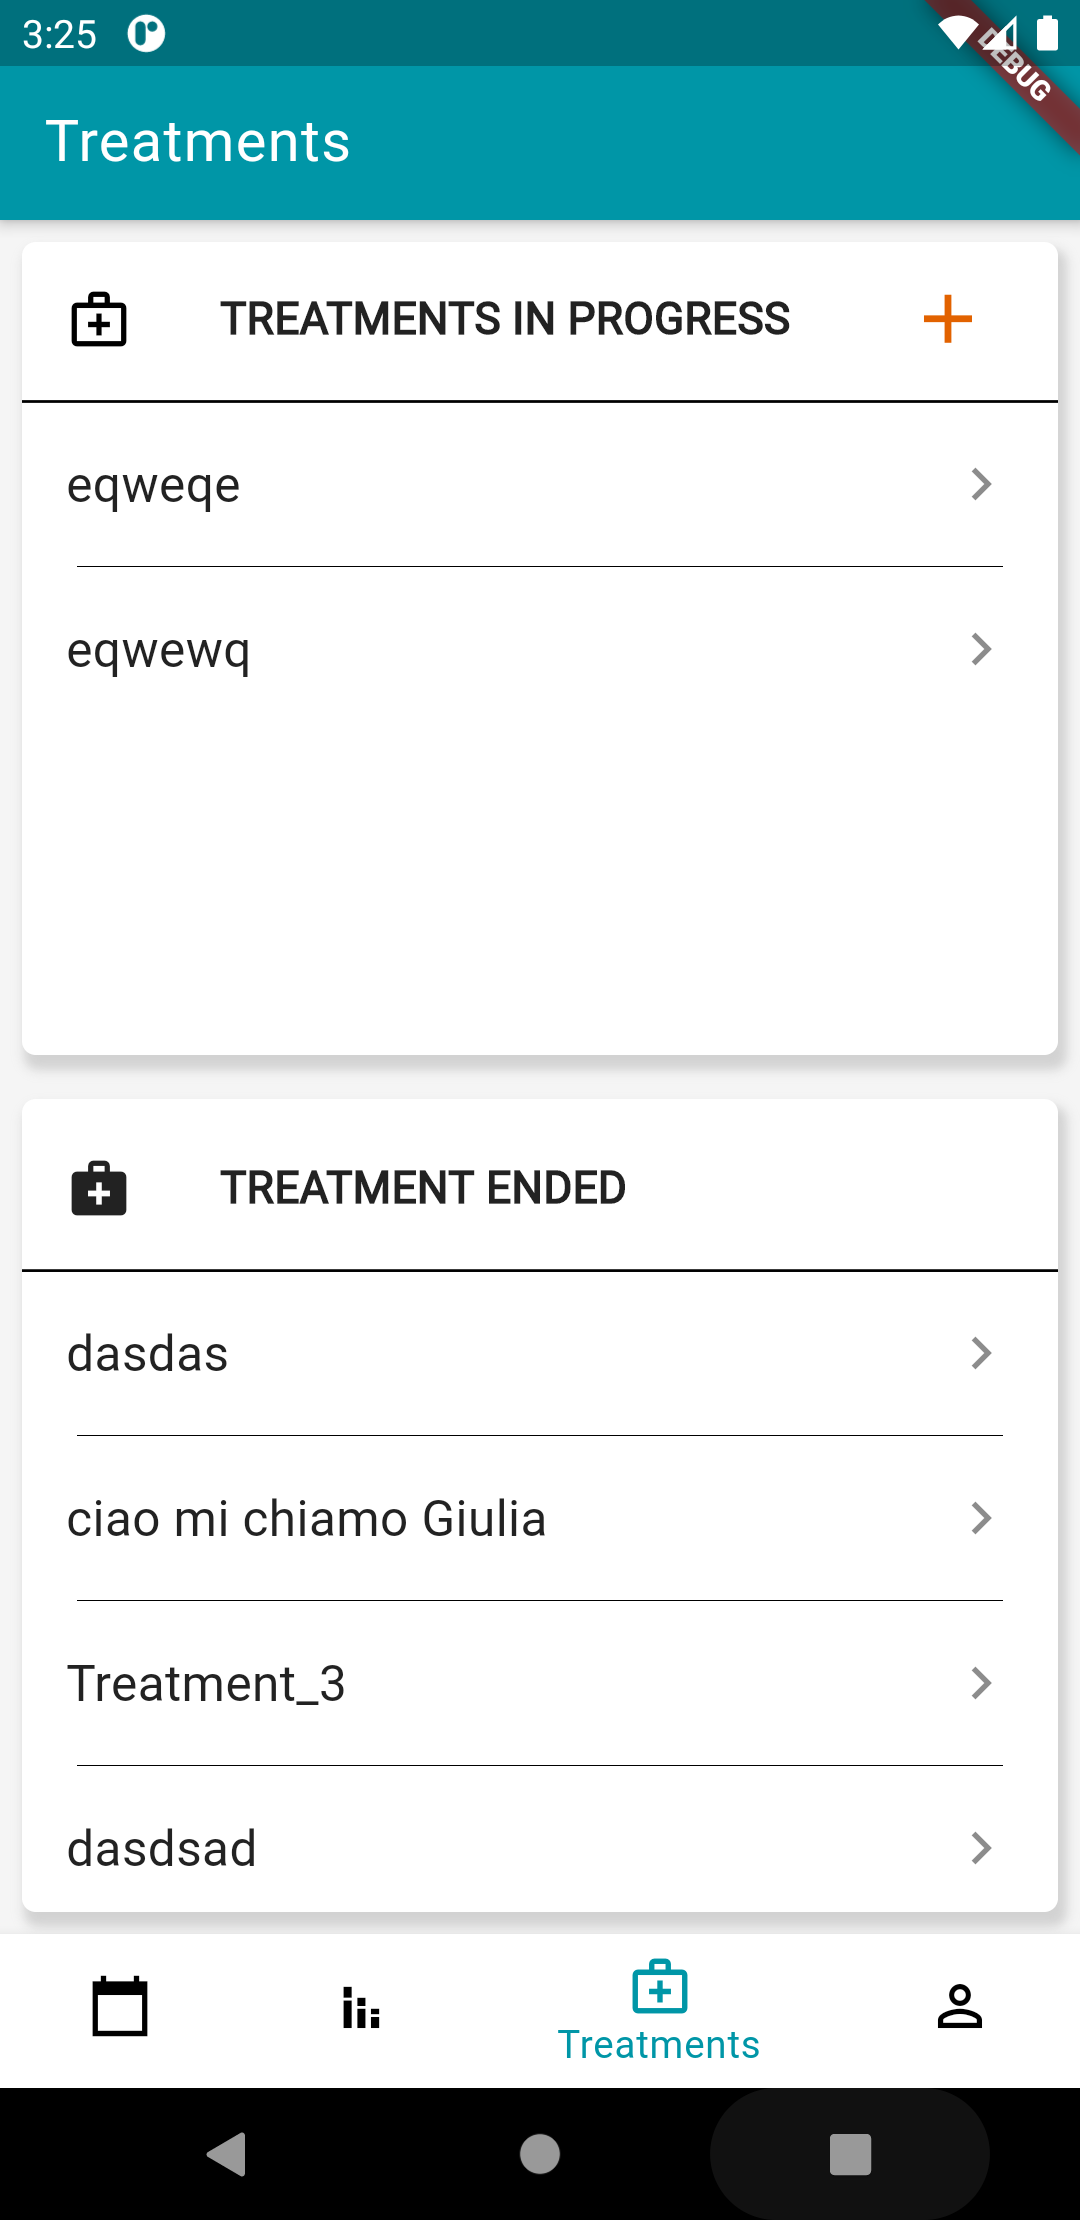
\includegraphics[width=\linewidth]{treatments1.PNG}
\caption{\textbf{Treatments}}
\end{subfigure}\hfill
\begin{subfigure}[tr]{0.3\linewidth}
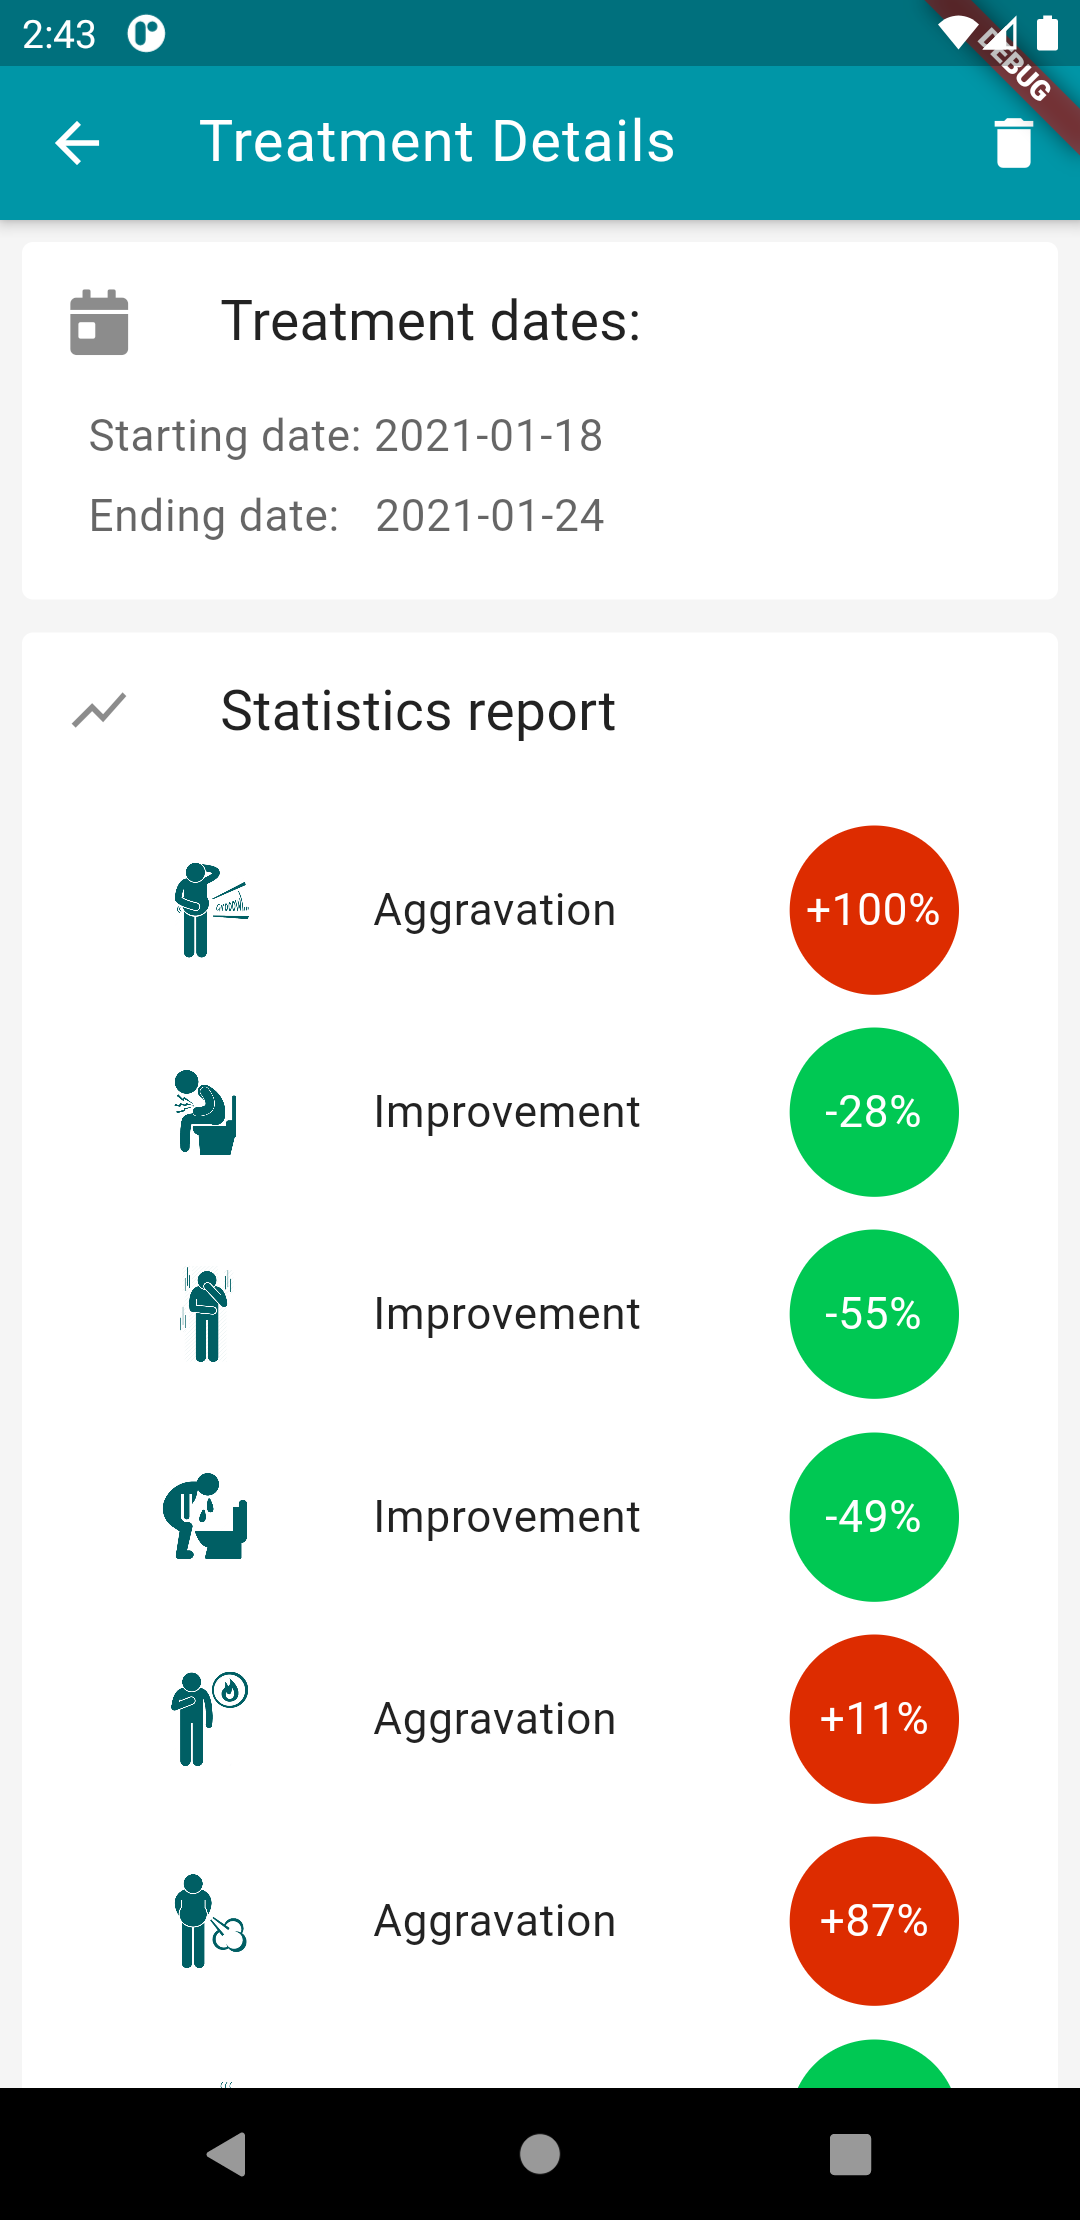
\includegraphics[width=\linewidth]{treatments2.PNG}
\caption{\textbf{Completed }}
\end{subfigure}
\hspace*{\fill}
\begin{subfigure}[tr]{0.3\linewidth}
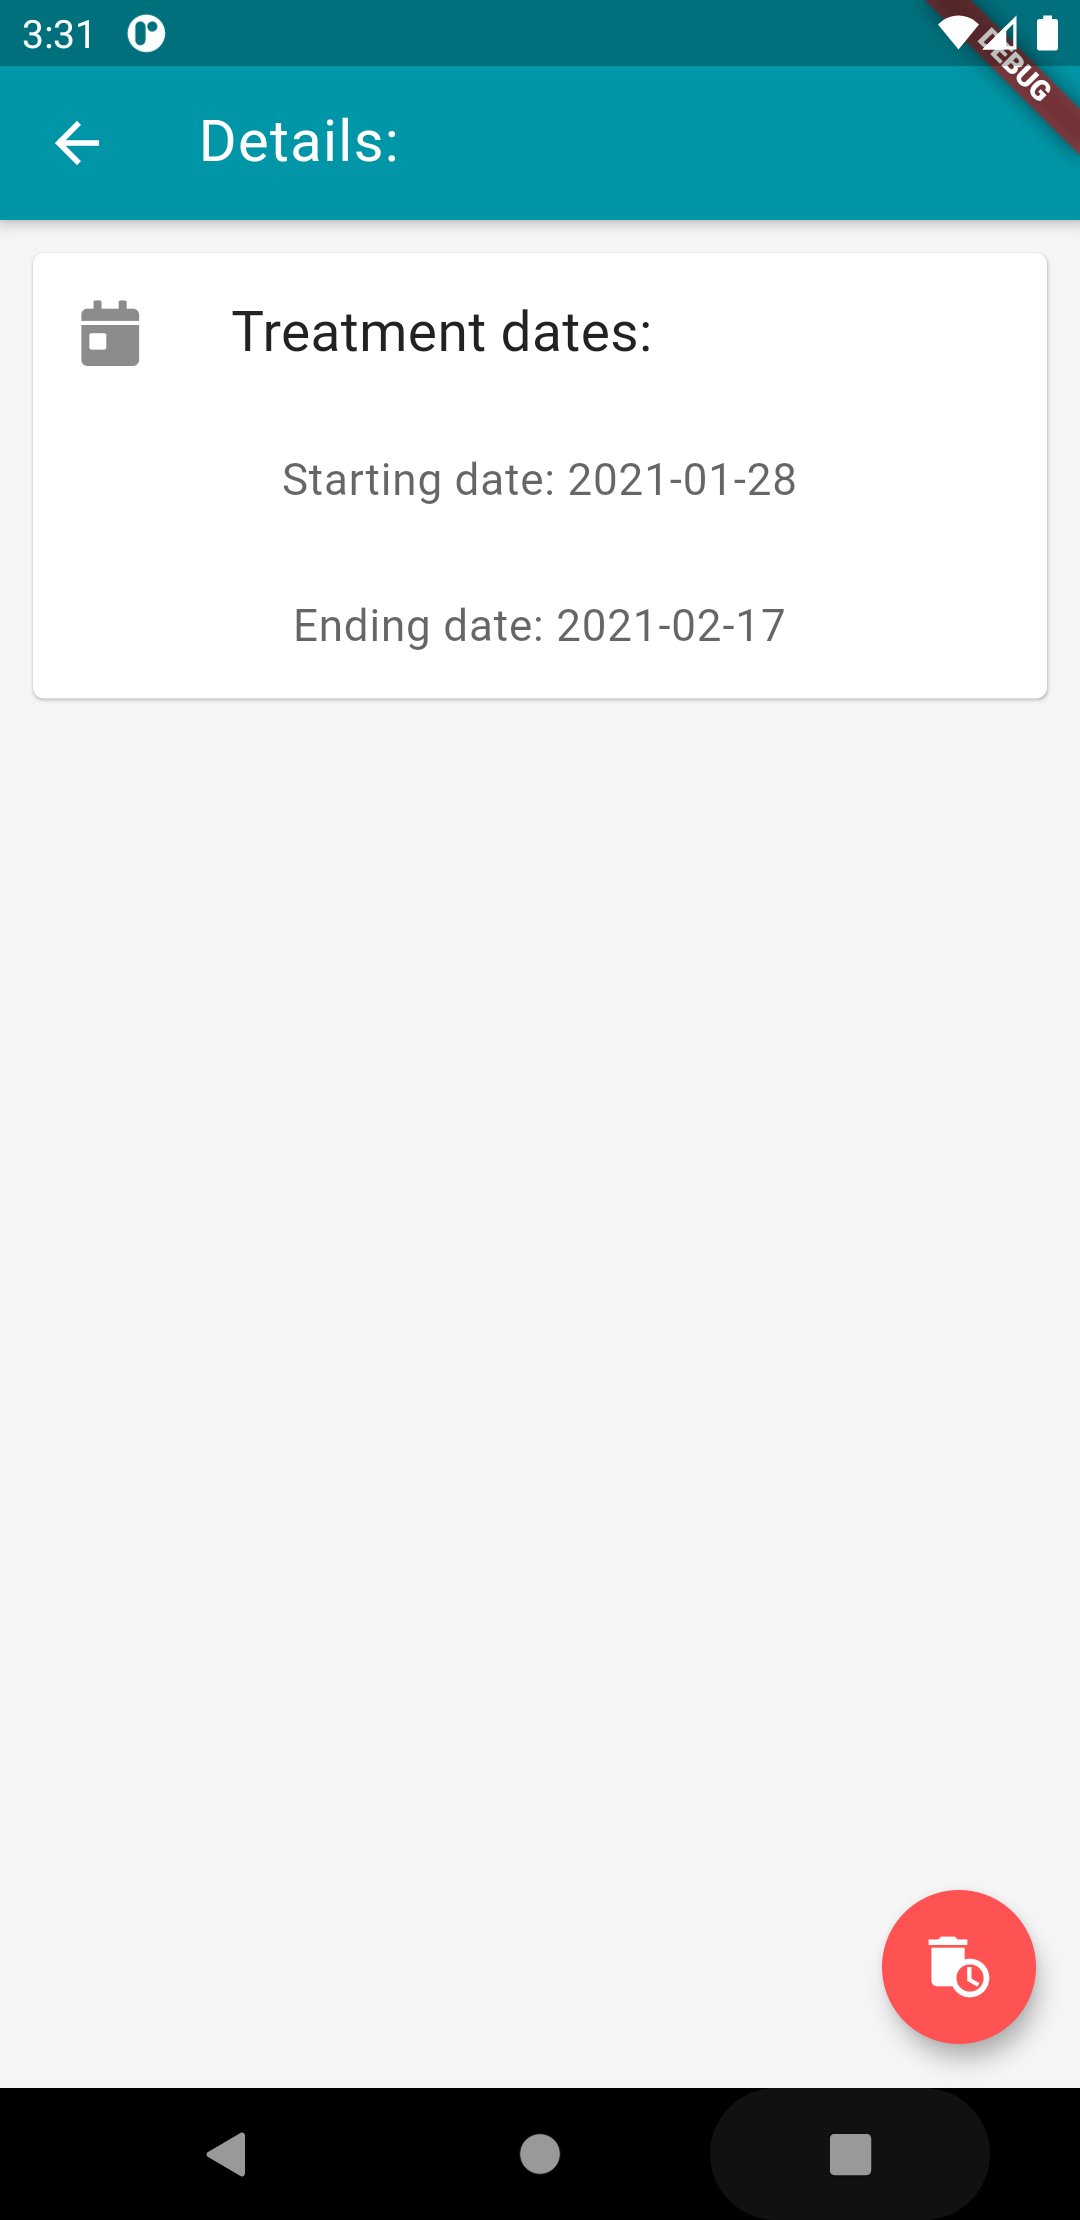
\includegraphics[width=\linewidth]{treatments3.PNG}
\caption{\textbf{In progress}}
\end{subfigure}
\hspace*{\fill}
\end{figure}
\begin{itemize}[•]
\item The treatment screen shows the user all their medical/dietary treatments: both those still in progress and those completed. 
\item By clicking on any treatment still in progress, the user will be able to view its details. 
\item If the user clicks on a completed treatment, in addition to the general information, he/she will also be shown the percentage progress of the symptoms: which ones have improved, which ones have worsened. The user can then assess the effectiveness or otherwise of that particular treatment. 
\end{itemize}
\clearpage

\item [ 7)Personal page]
\
\
\
\begin{figure}[h!]
\centering
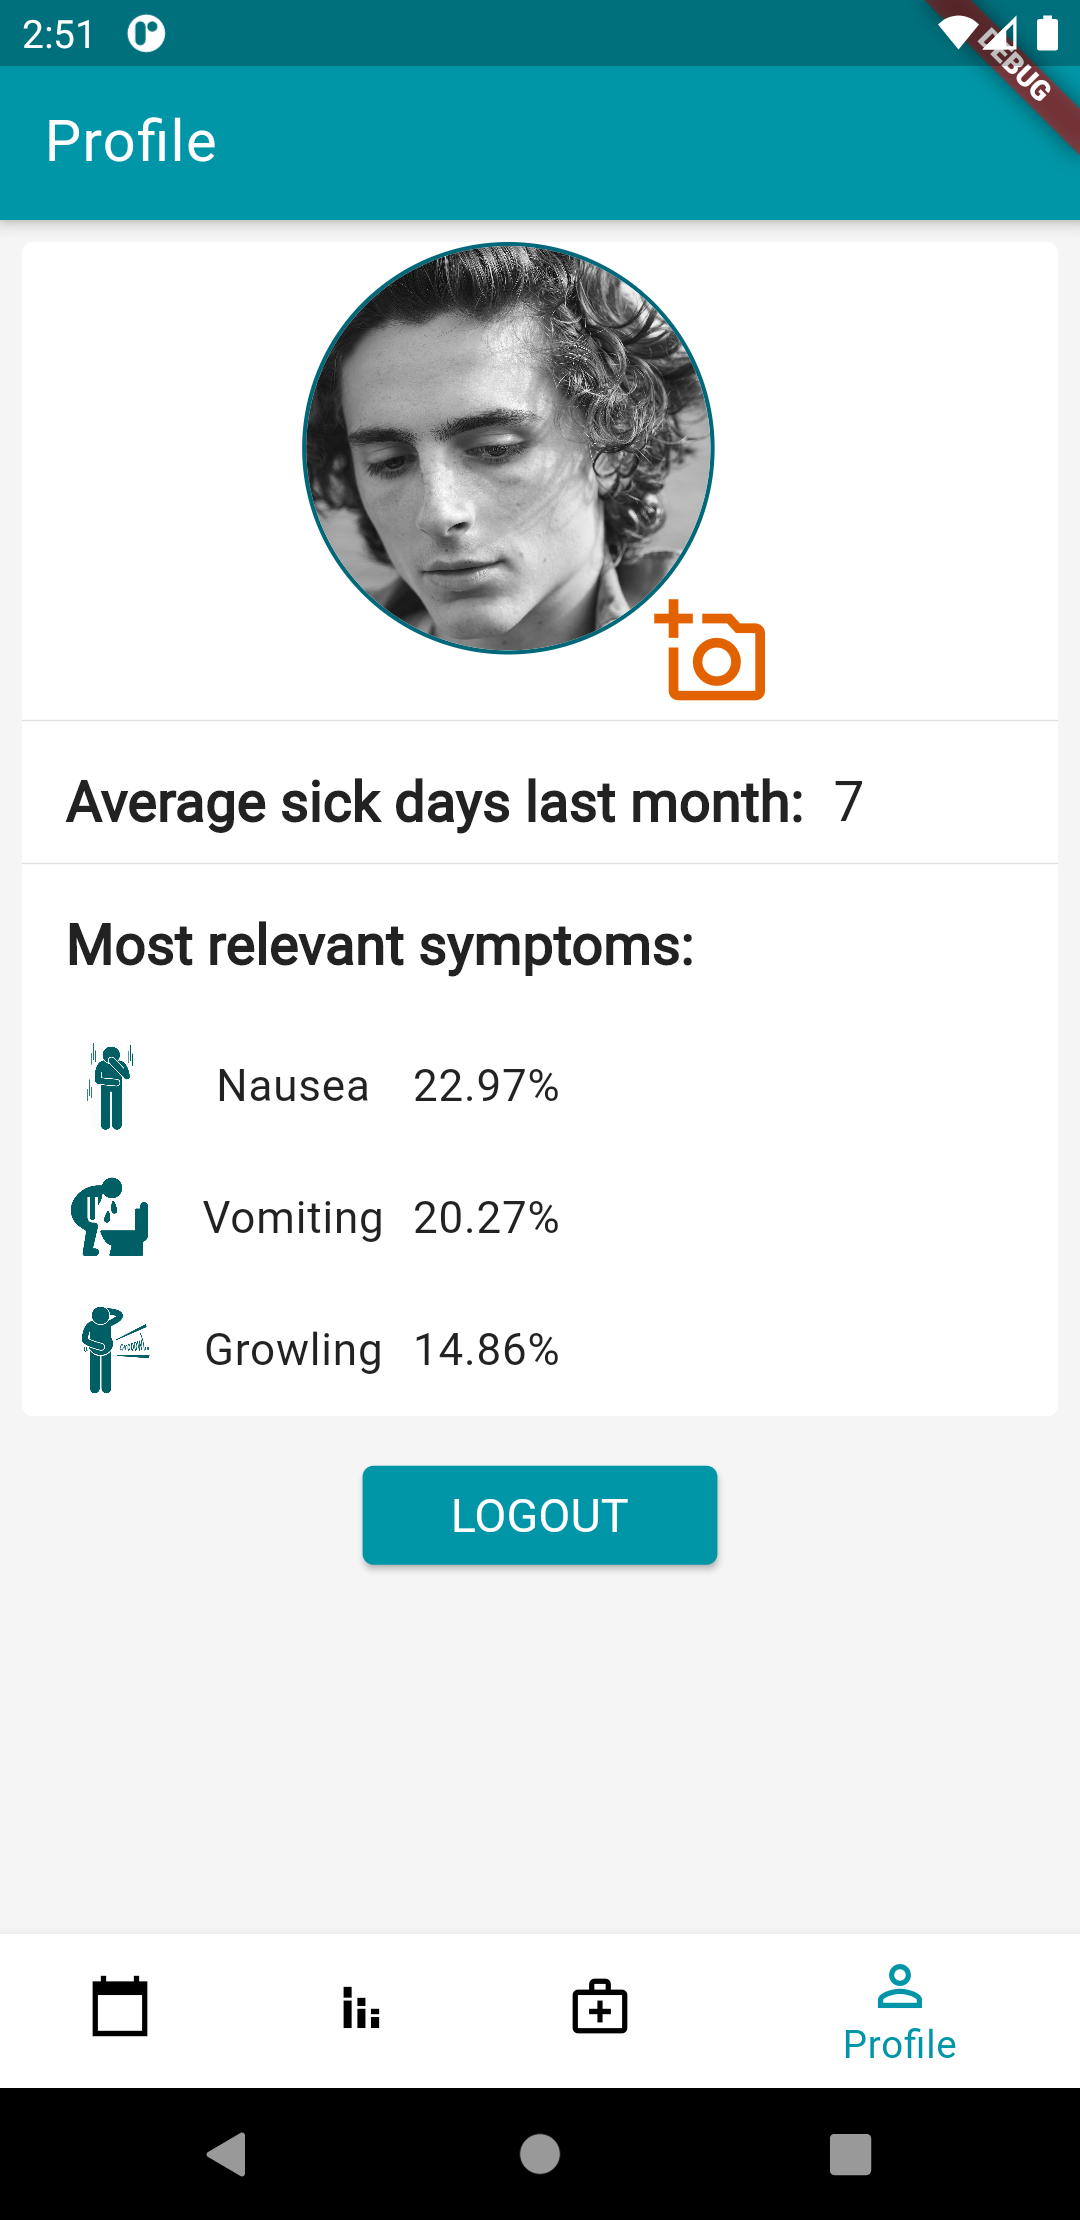
\includegraphics[width=6cm,height=12cm]{PersonalPage.PNG}
\end{figure}
\begin{itemize}[•]
\item The last screen concerns the user's personal information. The only action he can take is to add a profile picture. However, he can view some recap information since he started using the app: the average days he has been sickest with a severity value above 3 on a scale of one to ten and the 3 symptoms that have appeared most frequently.
\end{itemize}

\end{description}


\section{Implementation,Integration and Test Plan:}


\subsection{Integration Testing Strategy}
Flutter automated tests help ensure that app performs correctly before publish it.
Automated testing falls into a few categories:
\begin{itemize}[•]
\item A unit test tests a single function, method, or class.
\item A widget test tests a single widget.
\item An integration test tests a complete app or a large part of an app.
\end{itemize}
\subsubsection{Widget tests}
A widget test is more comprehensive than a unit test.
For example, the Widget being tested should be able to receive and respond to user actions and events, perform layout, and instantiate child widgets. For that reason, we have decided to perform some widget tests in order to testing the most main  functionality that the user can do in our appplication as adding a dish, a treatment, a symptom or removing them.
\begin{itemize}[•]
\item \textbf{Example:} add new symptom test\\
In this test we want to check that all the parameters required for the user to be able to add a new symptom on a given day have been entered. 
\begin{figure}[h!]
\centering
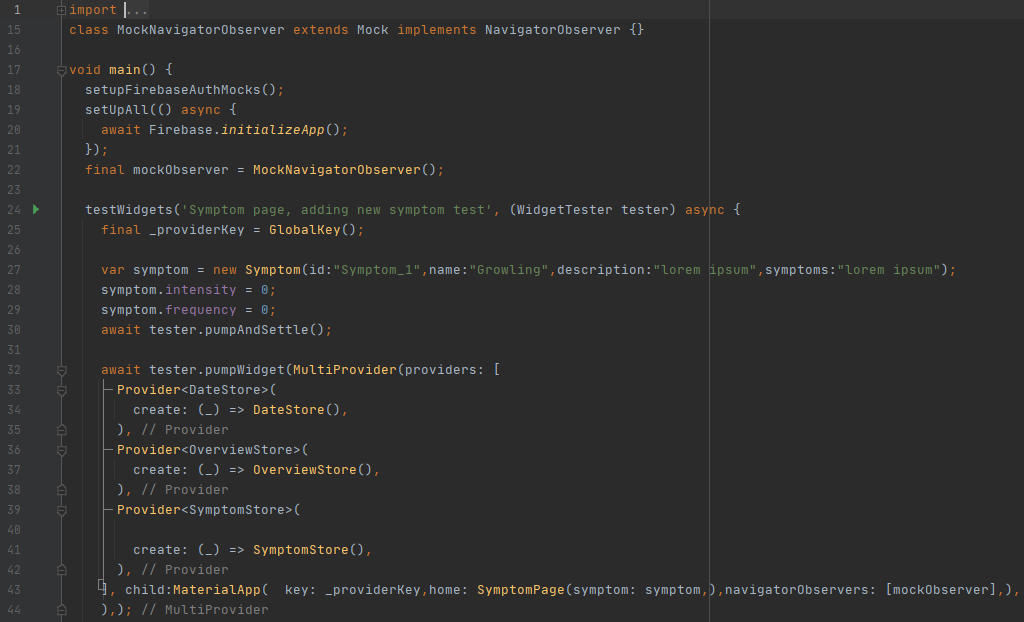
\includegraphics[width=\linewidth,height=8cm]{inizializzareSymptomPage.PNG}
\caption{Symptom page initialization}
\medskip
\small
The test requires the creation of an instance of the symptom and the initialization of the relevant page "SymptomPage" with the providers it uses.
\end{figure}
\\


\begin{figure}[h!]
\centering
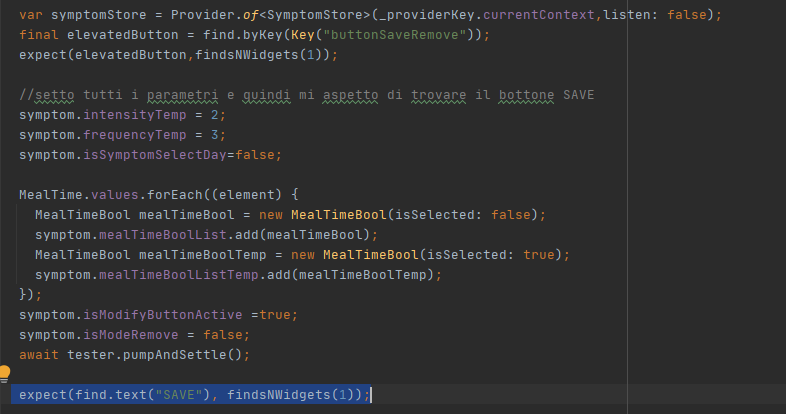
\includegraphics[width=\linewidth,height=8cm]{symptomButtonSave.PNG}
\caption{Setting symptom parameters}
\medskip
\small
Once the page has been initialized, we simulate user interaction and set various parameters to the symptom. We expect the Save button to become clickable.
\end{figure}

\begin{figure}[h!]
\centering
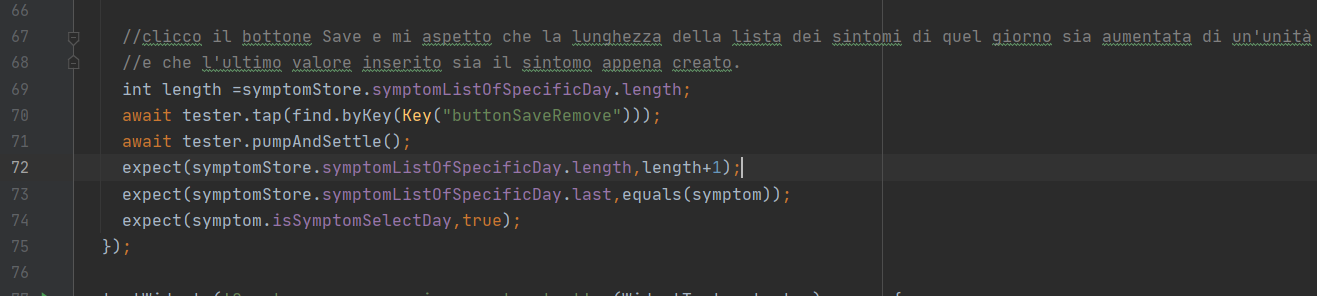
\includegraphics[width=\linewidth,height=4cm]{CreazioneSymptom.PNG}
\caption{Create new symptom}
\medskip
\small
After clicking the Save button, we expect the length of the symptom list for that day to have increased by one unit and the last value entered to be the newly created symptom.
\end{figure}

\end{itemize}


\clearpage
\subsubsection{Functional tests}
Our mobile app  needs to communicate with firebase and OpenFoodFacts databases. When we retrieve data from firebase store, we encapsule them in model classes like Dish, Symptom or Treatment in order to structure data. In order to do that we use jsonDecode() function (using the built-in JSON decoder in dart:convert).
\\
We pass the Firebase  JSON string  to the jsonDecode() function, and then looking up the values we need in the resulting Map<String, dynamic>. 
For example the Dish.fromJson() constructor, is used for constructing a new Dish instance from a map structure. \\
While, when we retrieve data from OpenFoodFacts, we use the package for flutter in order to  retrieve information about products, their ingredients and image with the function OpenFoodAPIClient.getProduct().
During the testing part of our project we decided to test the json serialization for the firebase data and to test the function provided by OpenFoodFacts.
\begin{itemize}[•]
\item \textbf{Example:} new dish istance creation test\\
In this test we want to check that all data retrieved from firebase DB are correctly encapsulated in our Dish class. 
\begin{figure}[h!]
\centering
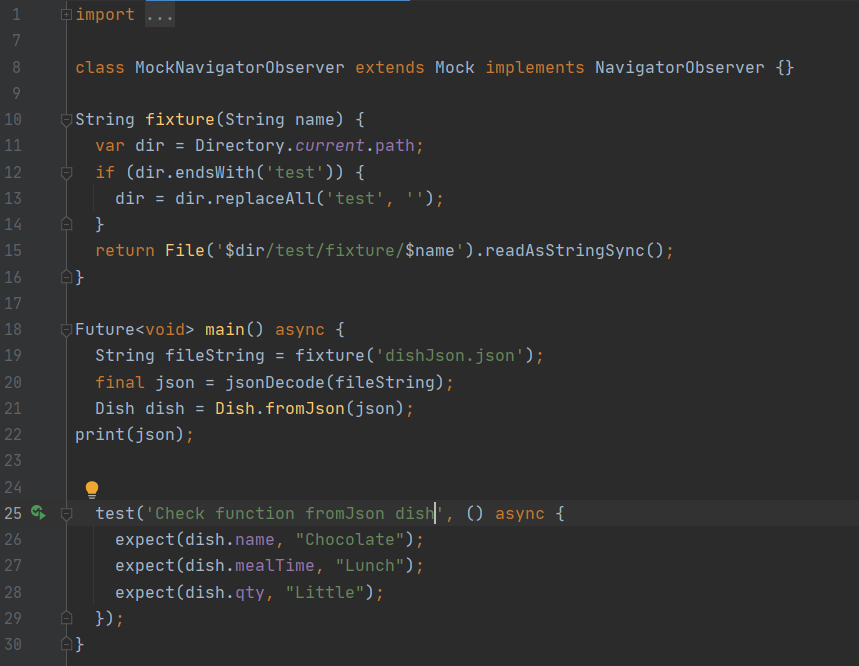
\includegraphics[width=\linewidth,height=10cm]{DishCreatedTest.PNG}
\caption{Creation of Dish istance}
\medskip
\small
\end{figure}
\end{itemize}


\subsection{Used Tools}
\begin{itemize}
\item StarUml 2.8.0
\item Miktex 2.9.6361
\item Texmaker 5.0.2
\item GitHubDesktop 1.0.6
\item AdobePhotoshop CC 2017
\item Power Point
\item Intellij
\end{itemize}
\end{document}